\phantomsection
%
%\addcontentsline{toc}{chapter}{ExperimentalEvaluation}
%
\chapter{Experimental Evaluation}
%
\markboth{ExperimentalEvaluation}{ExperimentalEvaluation}	% headings
%
\label{cap:experimental}
In this section the experiments performed to test the effectiveness of the \emph{Dynamic Checkpoint Rate Tuning} and the \emph{Reliam Resource Allocation Policy} will be examined and the results will be analyzed.
\section{Experimental setup}
We performed several experiments in order to evaluate the work proposed by this thesis. in order to test the \emph{Dynamic Checkpoint Tuning} and the CPU quota allocation component of the \emph{Reliam Resource Allocation Policy} we used a high-end workstation, having a quad-core processor \emph{Intel i7-3770} on an x86\_64 architecture. The computer is provided with a 32GB \emph{RAM} and runs a \emph{Linux} operating system, with kernel version 4.15.0.

In our experiments, we used \emph{benchmarks} as workload to evaluate pros and cons of our work and provide the reader with a guideline on the use of the proposed tools with respect to the use cases.

\subsection{The NAS Parallel Benchmark Suite}
The NAS Parallel Benchmark Suite (NPB) \cite{doi:10.1177/109434209100500306} is a benchmark suite developed by the NASA Advanced Supercomputing Division, designed to evaluate the performances of parallel supercomputers. It is composed of five kernels and three pseudo-applications, available in commonly-used programming models like MPI and OpenMP and in a variety of predefined problem sizes.
The five kernels of the suite are:
\begin{itemize}
\item IS - Integer Sort
\item EP - Embarrassingly Parallel 
\item CG - Conjugate Gradient
\item MG - Multi-Grid on a sequence of meshes 
\item FT - discrete 3D fast Fourier Transform
\end{itemize}
While the three pseudo applications are:
\begin{itemize}
\item BT - Block Tri-diagonal solver
\item SP - Scalar Penta-diagonal solver
\item LU - Lower-Upper Gauss-Seidel solver
\end{itemize}

In our experimental evaluation of the \emph{Dynamic Checkpoint Rate Tuning}, we exploited the three pseudo applications. We excluded from our tests classes S, W, A and B, due to their small problem size, which causes an execution time too short to be representative for the sake of our research. Conversely, we excluded classes E and F, respectively, the former for its too long execution time and the latter for limitations in terms of memory of the hardware at our disposal. In the end, we selected both class C and D to perform an analysis aware of different workloads and a diversity of execution times. 

\subsection{The PARSEC Benchmark Suite}
The PARSEC Benchmark Suite \cite{7849432} is a benchmark suite for multiprocessor systems firstly developed by Intel and Princeton University. It is composed by thirteen applications, whose domain and type of parallelization is summarized in Table~\ref{tab:parsec}.

\begin{table}
    \centering
    \begin{tabular}{|l|l|l|}
    \hline
    \rowcolor{lightblue}\textbf{BENCHMARK} & \textbf{DOMAIN} & \textbf{PARALLELIZATION}\\
    \hline
        \rowcolor{odd}Blackscholes & Financial Analysis & Data-parallel\\
        \rowcolor{even}Bodytrack & Computer Vision & Pipeline \\
        \rowcolor{odd}Canneal & Engineering & Data-parallel  \\
        \rowcolor{even}Dedup & Enterprise Storage & Pipeline  \\
        \rowcolor{odd}Facesim & Animation & Data-parallel \\
        \rowcolor{even}Ferret & Similarity Search & Pipeline \\
        \rowcolor{odd}Fluidanimate & Animation & Data-parallel \\
        \rowcolor{even}Freqmine & Data Mining & Data-parallel \\
        \rowcolor{odd}Raytrace & Data Mining & Data-parallel \\
        \rowcolor{even}Streamcluster & Financial Analysis & Data-parallel \\
        \rowcolor{odd}Swaptions & Media Processing & Data-parallel \\
        \rowcolor{even}Vips & Media Processing & Pipeline \\
        \hline
    \end{tabular}
    \caption{Workload of PARSEC benchmarks \cite{princetonuniversity}.}
    \label{tab:parsec}
\end{table}

Each benchmark is provided with three sets of inputs, intended, respectively, for testing, simulation and execution on real machines. Benchmarks are also provided with large working sets, even with a relatively constrained input set \cite{7849432}, which grow either proportionally to the data set size or to the number of cores.

For our experimental evaluation of the mathematical model behind the quota assignment of the Reliam Resource Allocation Policy, we used the Fluidanimate PARSEC benchmark, launched with 2 threads processing 400 frames of the \emph{native} input set, i.e. the one intended for real machines. The choice of a contained number of thread allowed us to observe the behavior of the modified PID controller in all three cases of quota allocation output:  scarce, in excess and approximately correct.

\subsection{Data Center Workload and Resource Management Simulator}
\label{sec:dcworms}
The Data Center Workload and Resource Management Simulator (DCworms) is an event-driven simulation tool, written in Java, which enables modeling and simulation of computing infrastructures to estimate their performance, energy consumption and energy efficiency metrics for diverse workloads and management policies \cite{DCworms}. DCworms allows a big margin of customization with respect to workload and computational resources modeling, providing the possibility of plugging in thermal, power and reliability models. It offers a multi-level description of the incoming jobs, whose abstraction level is depicted in Figure~\ref{fig:tasks}.
\begin{figure}
    \centering
    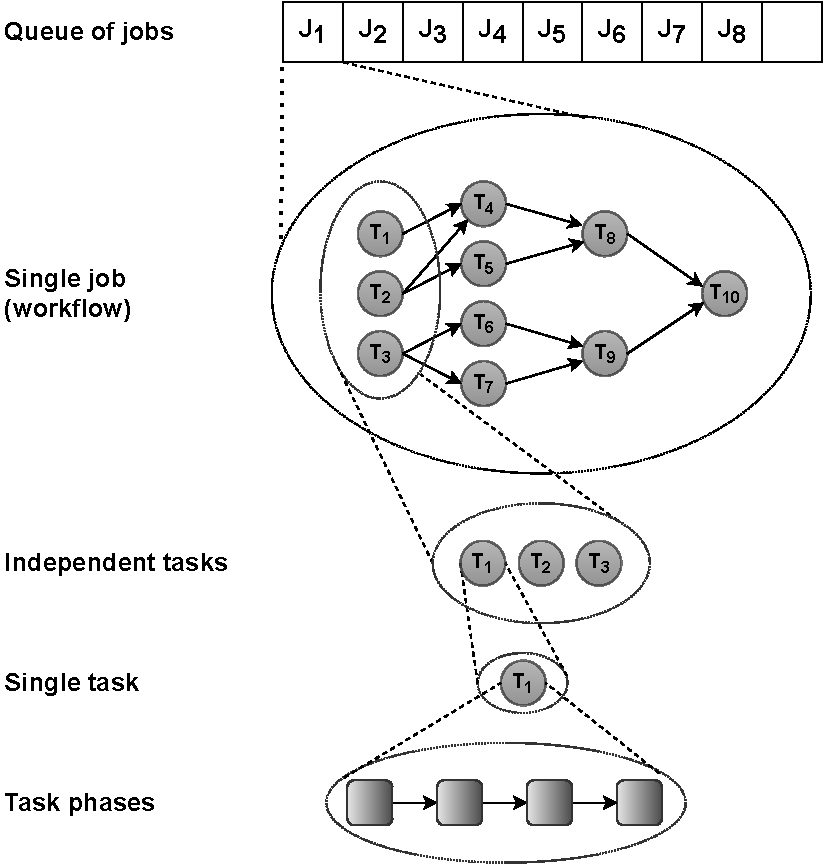
\includegraphics[width=0.8\textwidth]{dcworms_task.pdf}
    \caption{Levels of information about jobs in DCworms \cite{DCworms}.}
    \label{fig:tasks}
\end{figure}
Each task is described as a sequence of phases, periods of time in which the system is stable in terms of load, network and memory, in which the impact on the resources is observable. A simulated value representing the resource consumption profile is linked to each phase. 

In this thesis, we used DCworms to simulate the effect of the reliability-aware decisions performed by the \emph{Reliam Resource Allocation Policy} on a multi-node scale. We plugged a reliability model in the simulator linearly dependent on the temperature, which, in turn, has been modeled as dependent on the CPU load.

More specifically, the temperature profile is modeled as described by Leva et al. in \cite{leva2018}:
\begin{enumerate}
    \item The thermal state is updated:
    \begin{flalign*}
    &state = (0.03 * state + 22 * timeStep * cpuLoad) / (timeStep+ 0.03)&
\end{flalign*}
    \item The current temperature is computed:
    \begin{flalign*}
        & temp = state + 30&
    \end{flalign*}
\end{enumerate}

Given the function \verb|GetTemperature()|, implementing the thermal model, the reliability value is computed as described in Algorithm~\ref{alg:rel_model}.

\begin{algorithm}
    \SetKwInput{KwInput}{Input}
    \SetKwInput{KwConstant}{Constant}% Set the Input
    \SetKwInput{KwOutput}{Output}              % set the Output
    \DontPrintSemicolon
    \BlankLine

    \KwInput{CPU load \emph{cpuLoad}}
    \KwInput{Last observed thermal state \emph{state}}
    \KwInput{Random number \emph{rand}}
    \KwConstant{Stress temperature \emph{tStress}}
    \KwOutput{Reliability level \emph{rel}}
    %\BlankLine
    \algrule
    

\BlankLine
\SetKwFunction{Funcs}{GetReliability}
\SetKwProg{Fn}{double}{:}{}
\Fn{\Funcs{\KwSty{int} cpuLoad, \KwSty{float} rand, \KwSty{float} state}}{

\KwSty{float} temp = GetTemperature(cpuLoad, state)\;
    \KwSty{double} rel = (1-temp/tStress)*(1-rand)\;
    \KwRet rel\;
 }
    \BlankLine
   \caption{Reliability model implementation.}
   \label{alg:rel_model}
\end{algorithm}


We set $100^\circ$C as stress temperature, while using the \emph{rand} term to model the increase of the slope in the reliability curve after a certain threshold. More specifically, we defined the \emph{criticality threshold} as the percentage X such that:
\begin{align*}
    \begin{cases}
        0<rand<1 & \qquad \text{if }\frac{temp}{tStress}*100 \geq X\\
        \noalign{\vskip6pt}
        rand = 0 &\qquad \text{otherwise}
    \end{cases}
\end{align*}

\section{Dynamic Checkpoint Rate Tuning}
As deeply examined in {\hyperref[sec:dcrt]{Section~\ref{sec:dcrt}}}, aim of the Dynamic Checkpoint Rate Tuning is to tune an application specific interval between two consecutive checkpoints in order to meet time requirements and/or reliability goals. In order to test the effectiveness of our solution in different scenarios, we designed our model as explained in the following.

Given an application, we define its total time $T_{TOT}$ as: 
\begin{align}\label{eq:1}
    T_{TOT} = T_{exc\_tot} + T_{chk\_tot}
\end{align}

where \(T_{exc\_tot}\) and \(T_{chk\_tot}\) are, respectively, the time passed executing the code of the application and the time passed performing checkpoints. Considering the existence of a constant hazard function $h(z) = \lambda$, defined as the rate of occurrence of a failure in an hour, and given $R(t)$, a function that outputs the time passed between the last available checkpoint and the restart of the application, we can formulate $T_{failure}$, the additional time spent in case of failure, and build the following system of equations:  
\begin{align}\label{eq:2}
    \begin{cases}
    T_{TOT} = T_{exc\_tot} + T_{chk\_tot}\\
    \noalign{\vskip9pt}
    T_{failure} =  \displaystyle\int_0^{T_{TOT}}\lambda * R(t)dt
    \end{cases}
\end{align}
$R(t)$ is, in turn, composed by $T_{rst}$, the time spent restarting the application, and $T_{re\_exc}$, the time passed re-executing the piece of code whose execution was performed after the completion of the last checkpoint. Thus, we arrived at the following definition of $R(t)$:
\begin{align}\label{eq:3}
    R(t) = T_{rst}(t) + T_{re\_exc}
\end{align}
Since $T_{rst}$ mostly depends on human interaction and, in any case, does not depend on the logic of this component, we consider it negligible for the sake of this study, hence, from now on, we will simplify the computation of $R(t)$ as:
\begin{align}
    R(t) = T_{re\_exc}(t)
\end{align}

\begin{figure}[H]
    \centering
    \subfloat[\centering Benchmarks problem size class C.]{{\includegraphics[width=0.6\textwidth]{chk_mean_c.pdf} }}\\
    \vspace{1.1em}
    \subfloat[\centering Benchmarks problem size class D.]{{\includegraphics[width=0.6\textwidth]{chk_mean_d.pdf} }}
    \caption{Checkpoint mean time in seconds and standard deviation of the benchmarks used in the experimental evaluation.}
    \label{fig:chk_mean}%
\end{figure}
Running the benchmarks used for this experimental evaluation, we made sure that, for each of such applications, we could approximate the duration of a checkpoint routine with the arithmetic mean of all checkpoints. In Figure~\ref{fig:chk_mean} the checkpoint mean of each used benchmark is shown, displaying that standard deviation never exceeds the 10\% of the mean. This result has two turn ups: not only we can re-write, without any loss of information, $T_{chk\_tot}$ as $n* T_{chk\_mean}$, where $n$ is the total number of performed checkpoints, but also, for construction of the \emph{Dynamic Checkpoint Rate Tuning}, we can do the same approximation also for the period between two consecutive checkpoints, hence, we can write:
\begin{align}
    T_{exc\_tot} = n*(T_{period} - T_{chk\_mean}) + T_{end}
\end{align}  
where $T_{period}$ is the arithmetic mean of the time passed between the start of two consecutive checkpoints, while $T_{end}$ is the execution time between the last checkpoint and the end of the program.
Up to this point, we re-write the system of equations \ref{eq:2} as:
\begin{align}\label{eq:4}
    \begin{cases}
    T_{TOT} = n*(T_{period} - T_{chk\_mean}) + n*T_{chk\_mean} + T_{end}\\
    \noalign{\vskip9pt}
    T_{failure} =  \displaystyle\int_0^{T_{TOT}}\lambda * R(t)dt
    \end{cases}
\end{align}
 Without any loss of information, we can neglect the term $T_{end}$ from the equation, since its value is certainly less than a checkpoint period. Simplifying,
\begin{align}
    \begin{cases}
        T_{TOT} = n*T_{period}\\
        \noalign{\vskip9pt}
        T_{failure} = \displaystyle\int_0^{T_{TOT}}\lambda * R(t)dt
    \end{cases}
\end{align}
As mentioned above, we consider the time span between the start of two consecutive checkpoints approximable with the arithmetic mean given by $T_{period}$. Thanks to this approximation, it is possible to discretize the integral of $T_{failure}$ in a summation of integrals. Those integrals will be defined between $t_{start\_exc_i}$ and $t_{end\_exc_i}$, respectively the starting time and the ending time of the execution of the application code in period $i$. Since we approximated each period with $T_{period}$ and each checkpoint time with $T_{chk\_mean}$, we find that:
\begin{align}
    t_{end\_exc_i} - t_{start\_exc_i} = T_{period} - T_{chk\_mean} = T_{exc\_mean}\qquad \forall i 
\end{align}

Starting from the assumptions just made, the computation of $T_{failure}$ becomes:

\begin{align} 
T_{failure} & = \displaystyle\int_0^{T_{TOT}}\lambda\, R(t)dt \\
 \noalign{\vskip9pt}
 & = \sum_{i=1}^n \displaystyle\int_{t_{end\_exc_i}}^{t_{start\_exc_i}}\lambda \,t_idt_i\\
  \noalign{\vskip9pt}
 & = \sum_{i=1}^n\lambda\,\frac{t_i^2}{2}\,\Bigr|_{t_{start\_exc_i}}^{t_{end\_exc_i}}\\
  \noalign{\vskip9pt}
 & = n\, \lambda\,\frac{{T_{exc\_mean}}^2}{2}\label{eq:tfailure}
\end{align}
We performed our experiments on classes C and D of the three pseudo-applications of the NPB suite, BT, LU and SP. We set $k=0.02$ for class C and $k=0.2$ for class D problem size, where $k$ is the upper bound on the overhead set by the user for the application at issue, and we plotted $T_{failure}$ as defined in Equation~\ref{eq:tfailure}, varying $\lambda$. Then, we summed the obtained $T_{failure}$ to the total overhead produced by the checkpointing routine and we plotted this sum, as well, varying $\lambda$. Results of such measurements are shown in Figures~\multiref{fig:real_c}{fig:real_d}. Finally, in Figure~\ref{fig:real_perc}, the percentage overhead caused by the sum of checkpointing time and the time to recover from a failure, on the execution of the only application code is displayed, again, varying $\lambda$.

{\captionsetup[subfloat]{labelformat=empty}
\begin{figure}
    \centering
    {
    \subcaption[]{Benchmark: BT}
    \subfloat[\centering]{{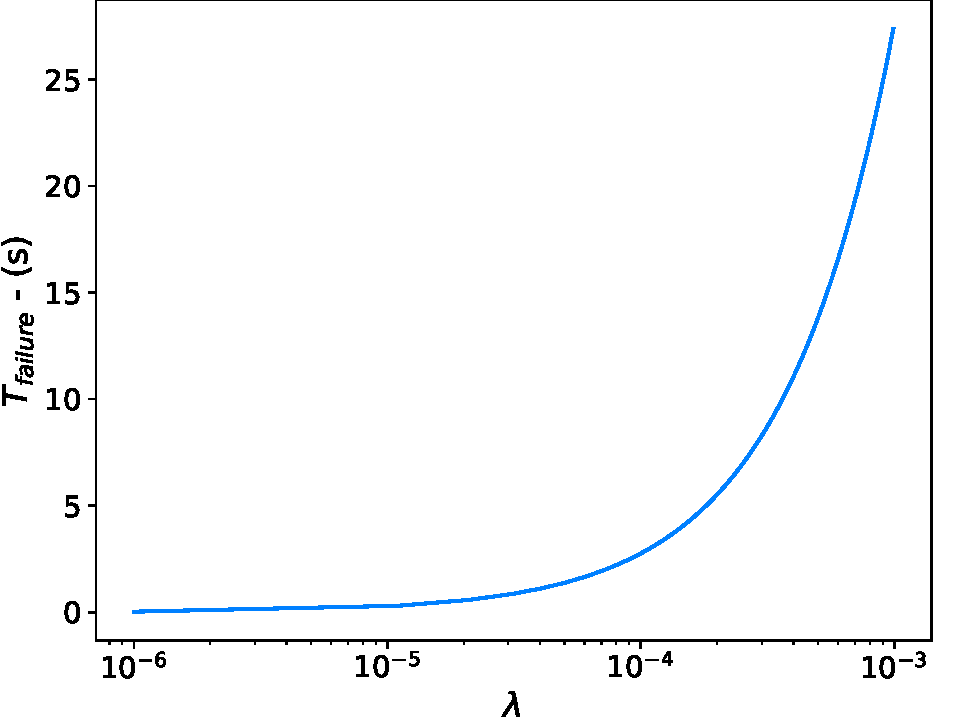
\includegraphics[width=0.49\textwidth]{avg_real_reset_time_BT_C.pdf} }}
    \subfloat[\centering]{{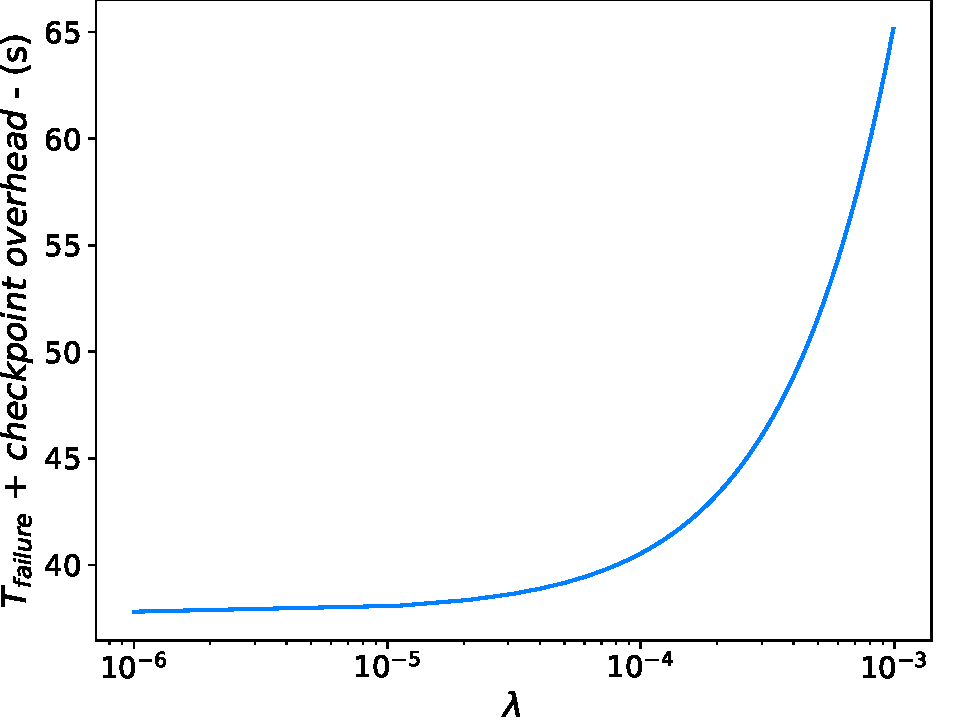
\includegraphics[width=0.49\textwidth]{avg_real_tot_ovhd_BT_C.pdf} }}\vspace{-1.1em}}
    {
    \subcaption[]{Benchmark: LU}
    \subfloat[\centering]{{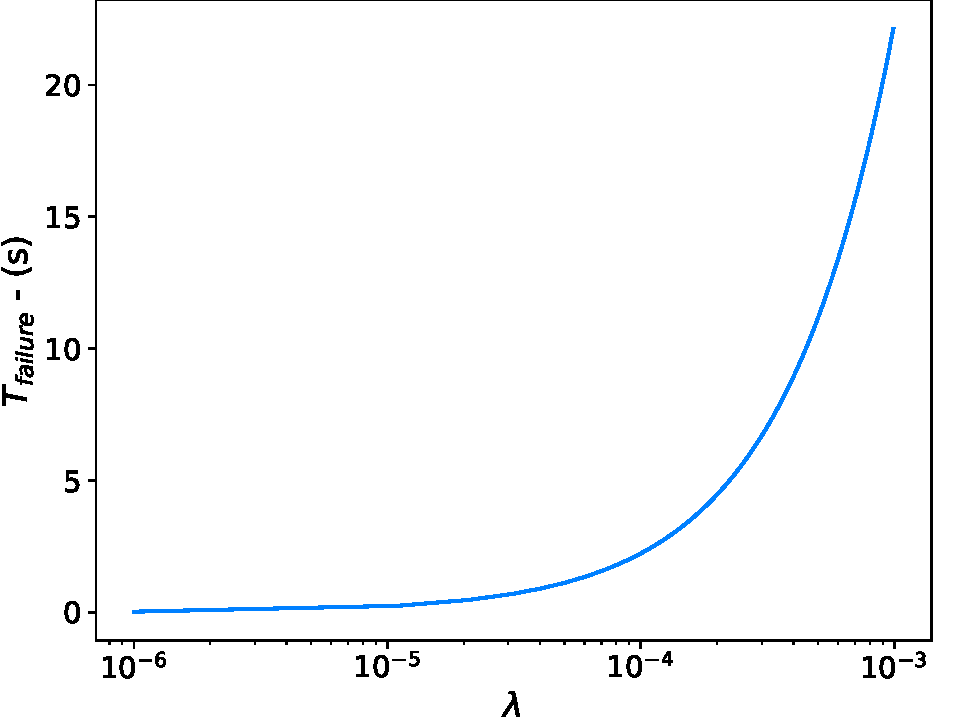
\includegraphics[width=0.49\textwidth]{avg_real_reset_time_LU_C.pdf} }}
    \subfloat[\centering]{{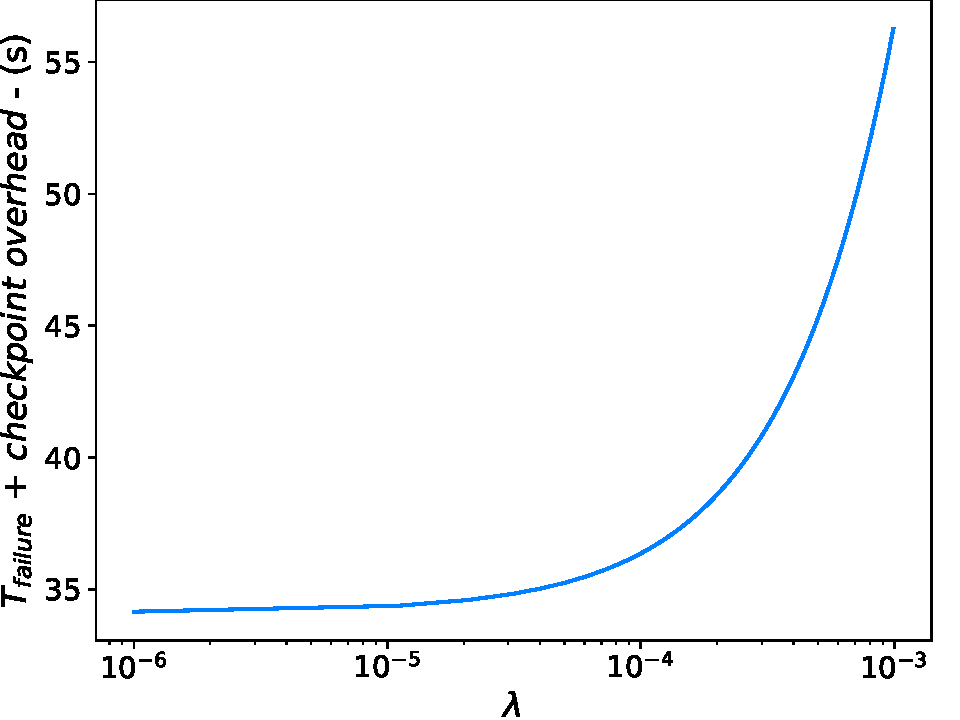
\includegraphics[width=0.49\textwidth]{avg_real_tot_ovhd_LU_C.pdf} }}\vspace{-1.1em}}
    {
    \subcaption[]{Benchmark: SP}
    \subfloat[\centering \textbf{(a)} Estimated mean overhead caused by the re-execution of application code in case of failure, varying $\lambda$.]{{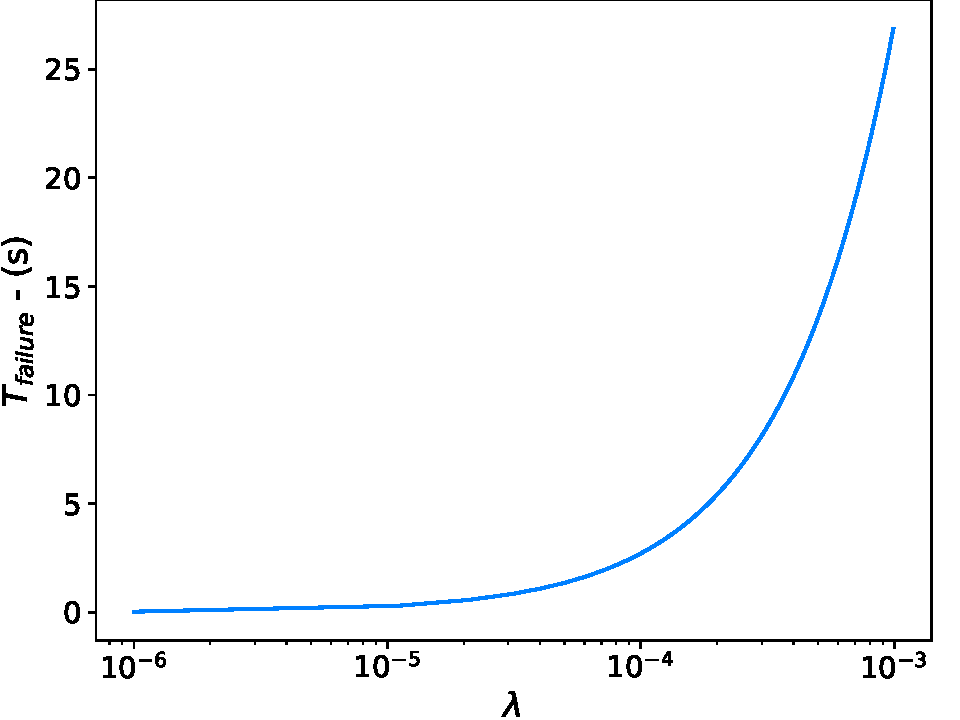
\includegraphics[width=0.49\textwidth]{avg_real_reset_time_SP_C.pdf} }}
    \subfloat[\centering \textbf{(b)} Sum of the value of \textbf{(a)} plus the checkpoint overhead, varying $\lambda$.]{{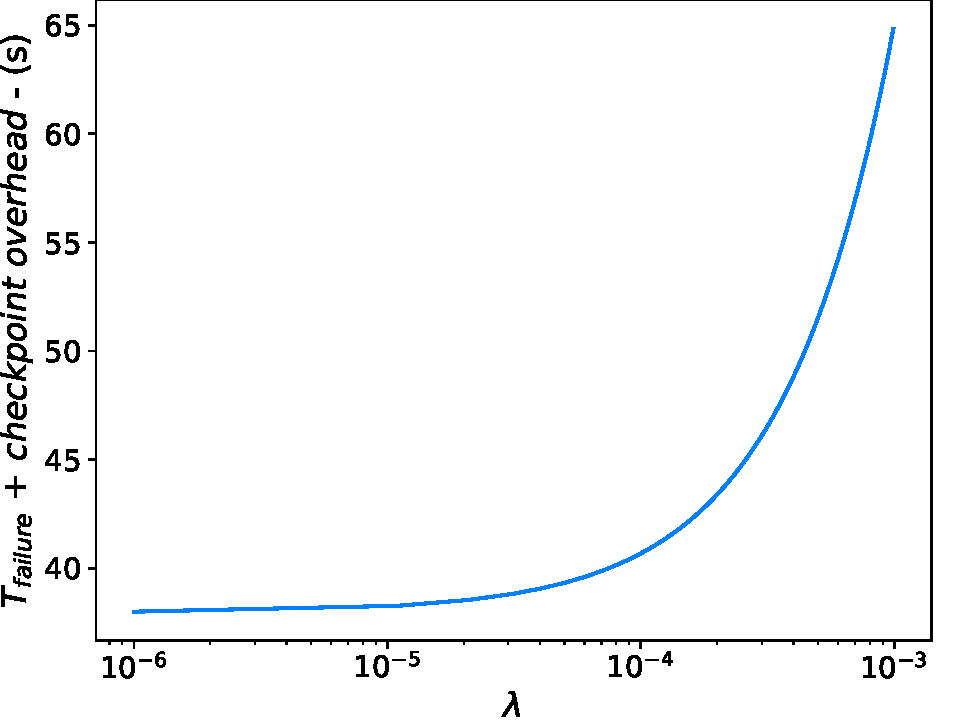
\includegraphics[width=0.49\textwidth]{avg_real_tot_ovhd_SP_C.pdf} }}}
    \caption{Plot of \textbf{(a)} $T_{failure}$, \textbf{(b)} $T_{failure}+checkpoint\ overhead$, varying $\lambda$ - Problem size class C, k=0.02, measurement in seconds.}%
    \label{fig:real_c}%
\end{figure}}

{\captionsetup[subfloat]{labelformat=empty}
\begin{figure}
    \centering
    {
    \subcaption[]{Benchmark: BT}
    \subfloat[\centering]{{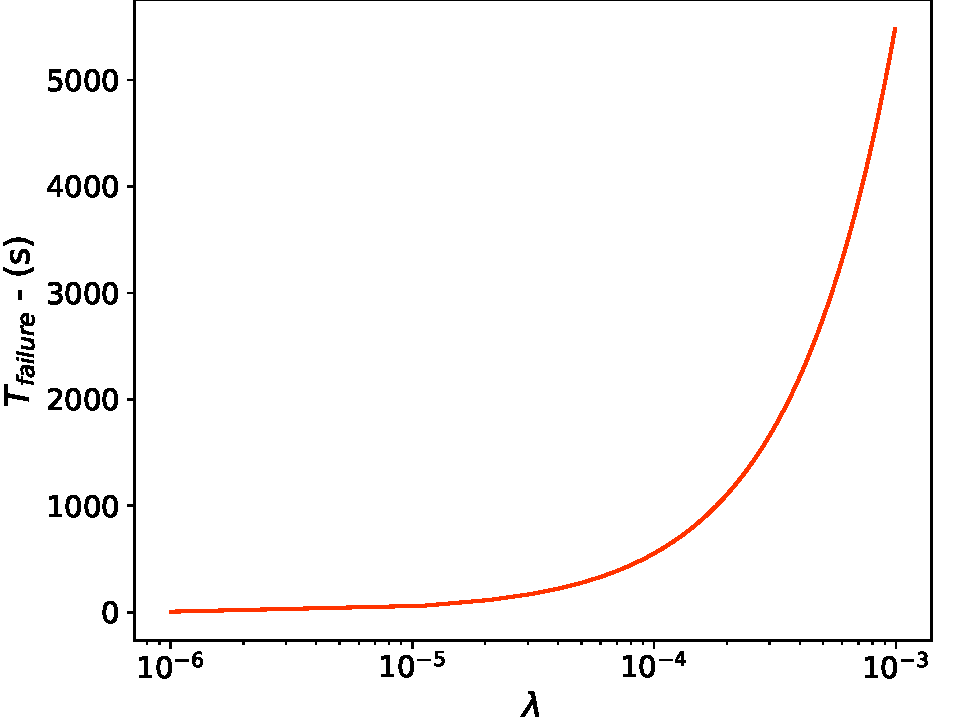
\includegraphics[width=0.49\textwidth]{avg_real_reset_time_BT_D.pdf} }}
    \subfloat[\centering]{{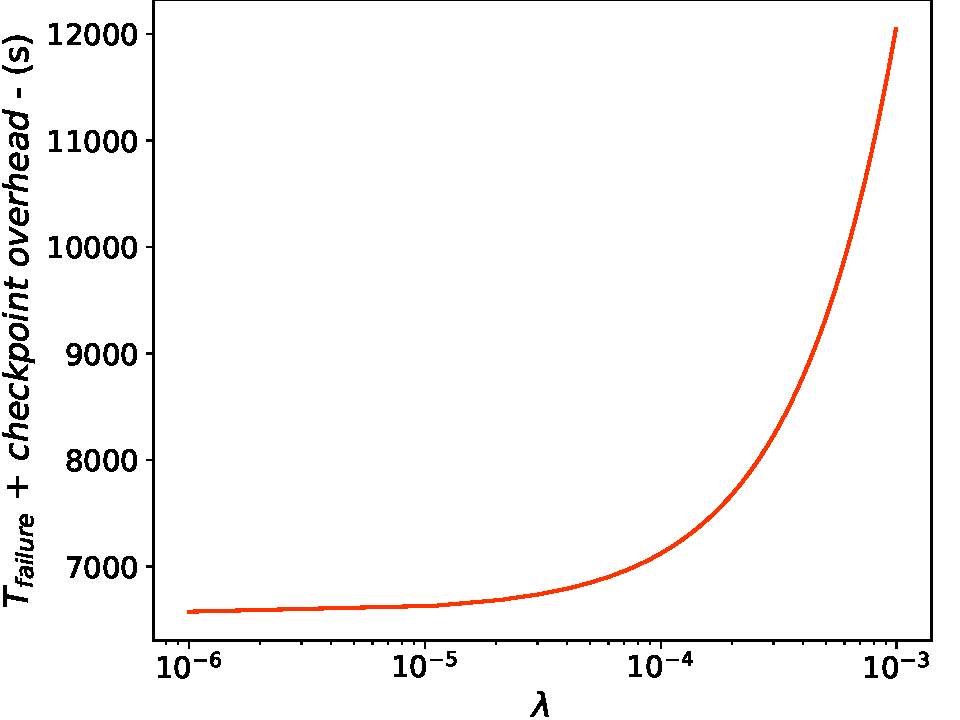
\includegraphics[width=0.49\textwidth]{avg_real_tot_ovhd_BT_D.pdf} }}\vspace{-1.1em}}
    {
    \subcaption[]{Benchmark: LU}
    \subfloat[\centering]{{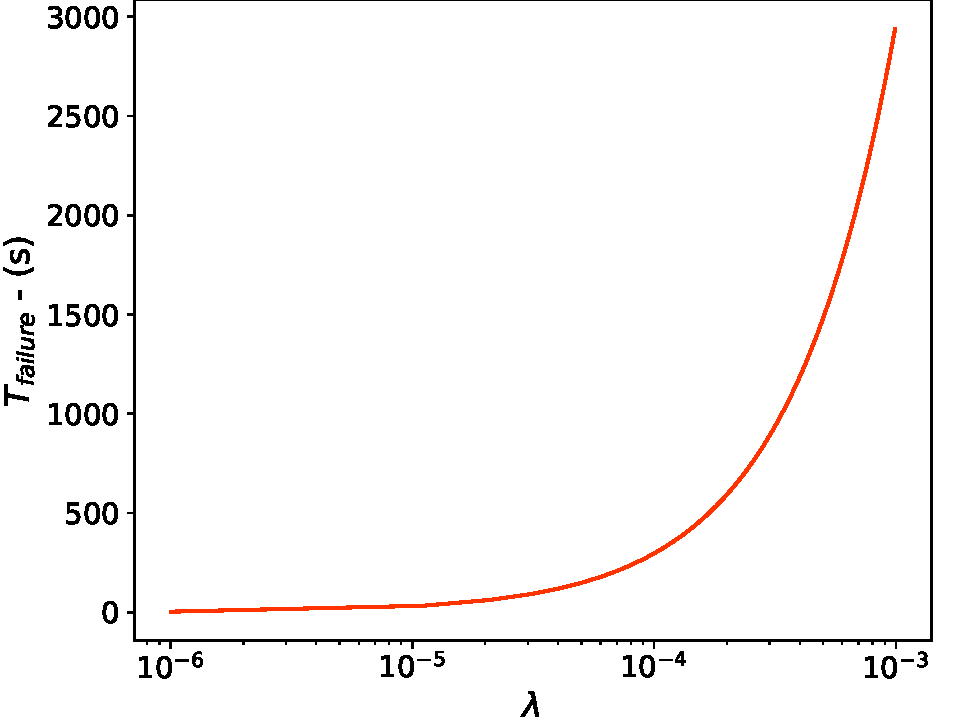
\includegraphics[width=0.49\textwidth]{avg_real_reset_time_LU_D.pdf} }}
    \subfloat[\centering]{{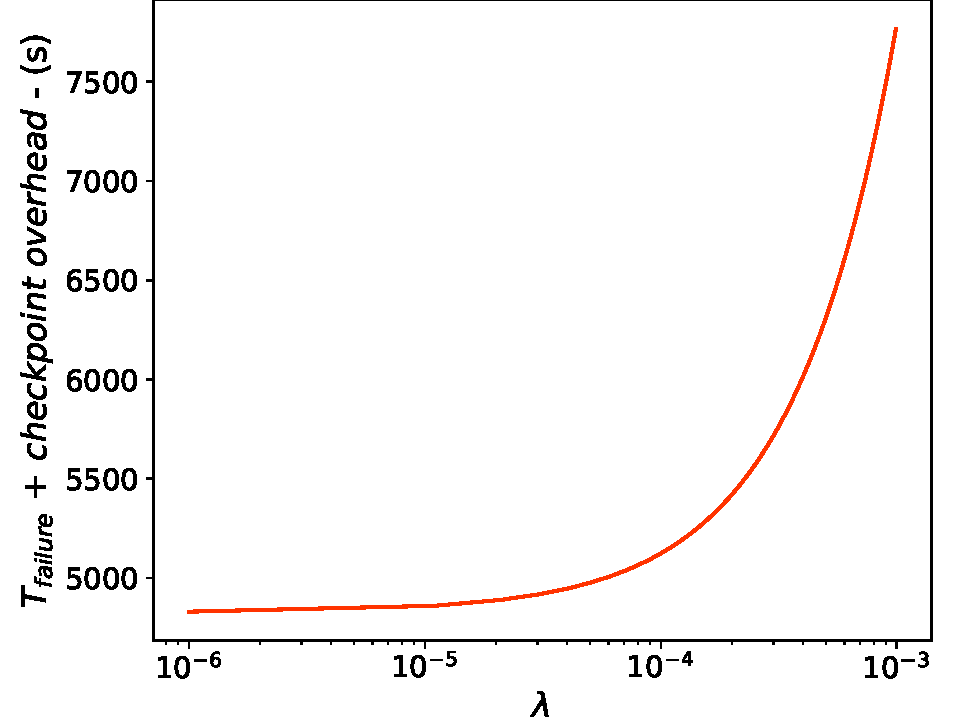
\includegraphics[width=0.49\textwidth]{avg_real_tot_ovhd_LU_D.pdf} }}\vspace{-1.1em}}
    {
    \subcaption[]{Benchmark: SP}
    \subfloat[\centering \textbf{(a)} Estimated mean overhead caused by the re-execution of application code in case of failure, varying $\lambda$.]{{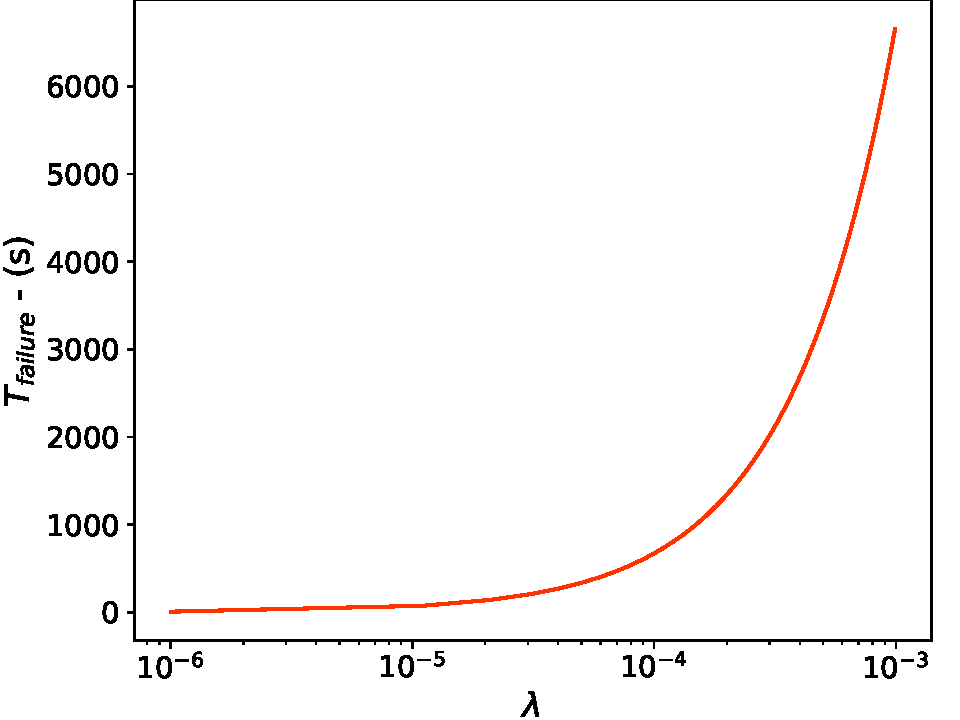
\includegraphics[width=0.49\textwidth]{avg_real_reset_time_SP_D.pdf} }}
    \subfloat[\centering \textbf{(b)} Sum of the value of \textbf{(a)} plus the checkpoint overhead, varying $\lambda$.]{{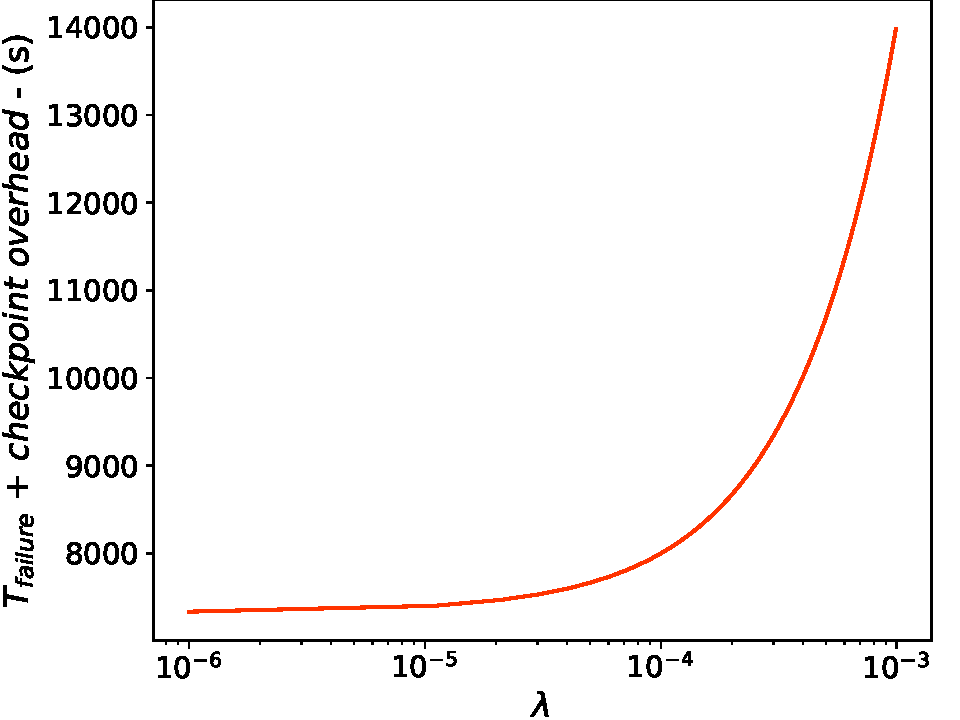
\includegraphics[width=0.49\textwidth]{avg_real_tot_ovhd_SP_D.pdf} }}}
    \caption{Plot of \textbf{(a)} $T_{failure}$, \textbf{(b)} $T_{failure}+checkpoint\ overhead$, varying $\lambda$ - Problem size class D, k=0.2, measurement in seconds.}%
    \label{fig:real_d}%
\end{figure}}

{\captionsetup[subfloat]{labelformat=empty}
\begin{figure}
    \centering
    {
    \subcaption[]{Benchmark: BT}
    \subfloat[\centering]{{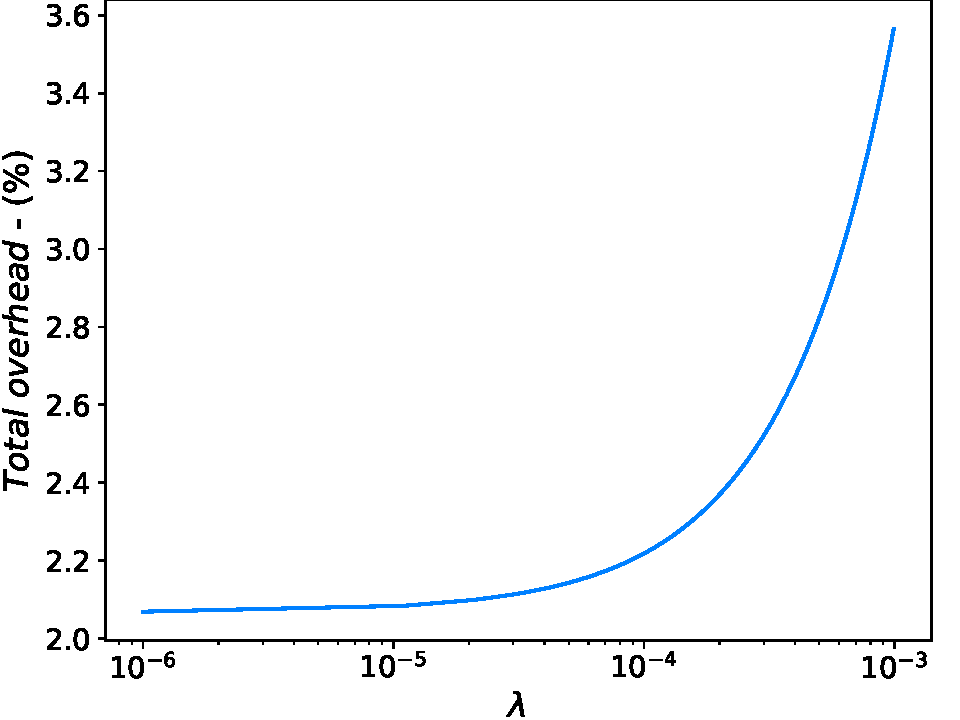
\includegraphics[width=0.49\textwidth]{real_perc_tot_ovhd_BT_C.pdf} }}
    \subfloat[\centering]{{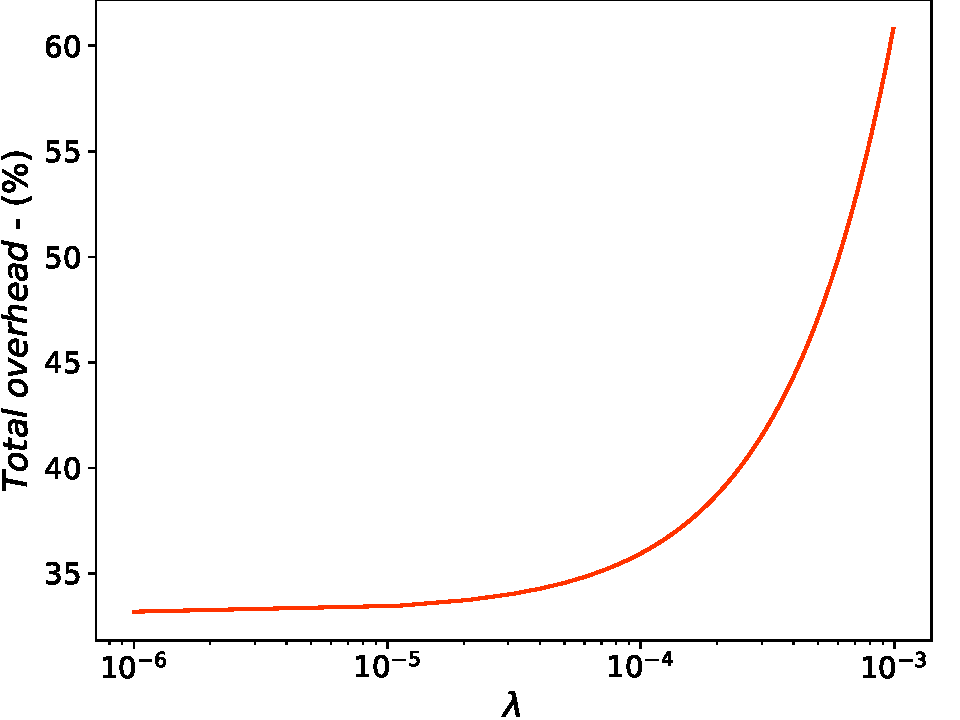
\includegraphics[width=0.49\textwidth]{real_perc_tot_ovhd_BT_D.pdf} }}\vspace{-1.1em}}
    {
    \subcaption[]{Benchmark: LU}
    \subfloat[\centering]{{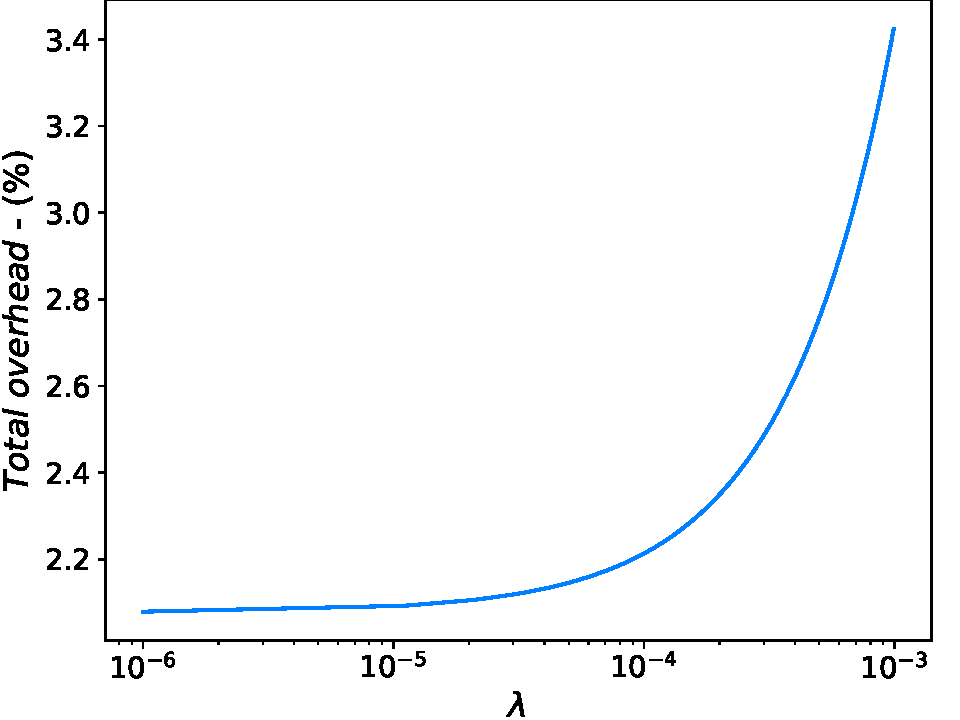
\includegraphics[width=0.49\textwidth]{real_perc_tot_ovhd_LU_C.pdf} }}
    \subfloat[\centering]{{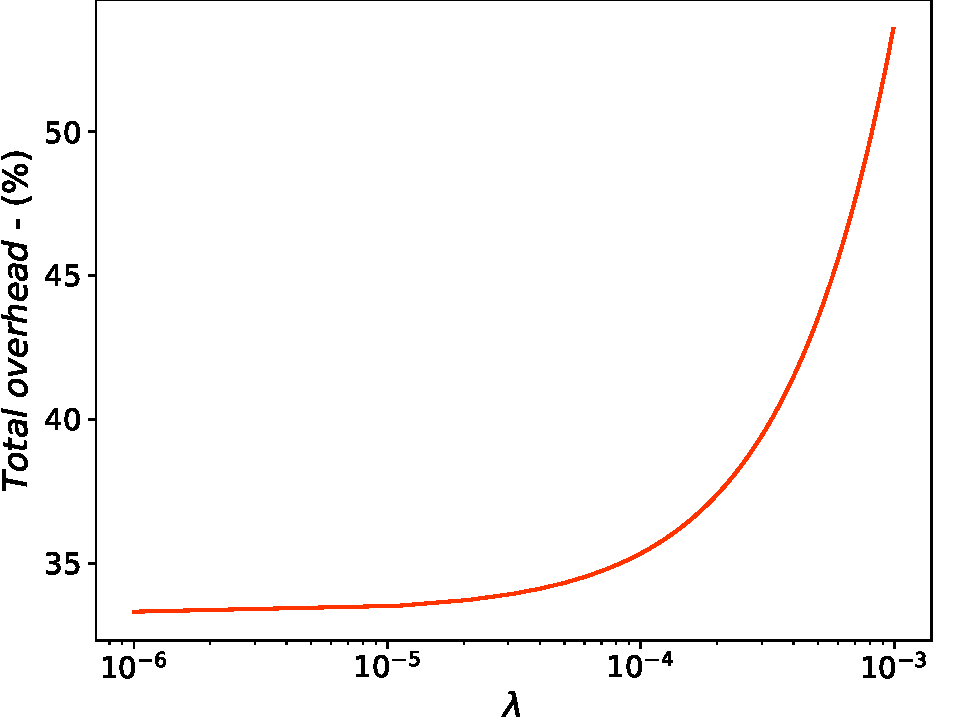
\includegraphics[width=0.49\textwidth]{real_perc_tot_ovhd_LU_D.pdf} }}\vspace{-1.1em}}
    {
    \subcaption[]{Benchmark: SP}
    \subfloat[\centering \textbf{(a)} Problem size class C - $k=0.02$.]{{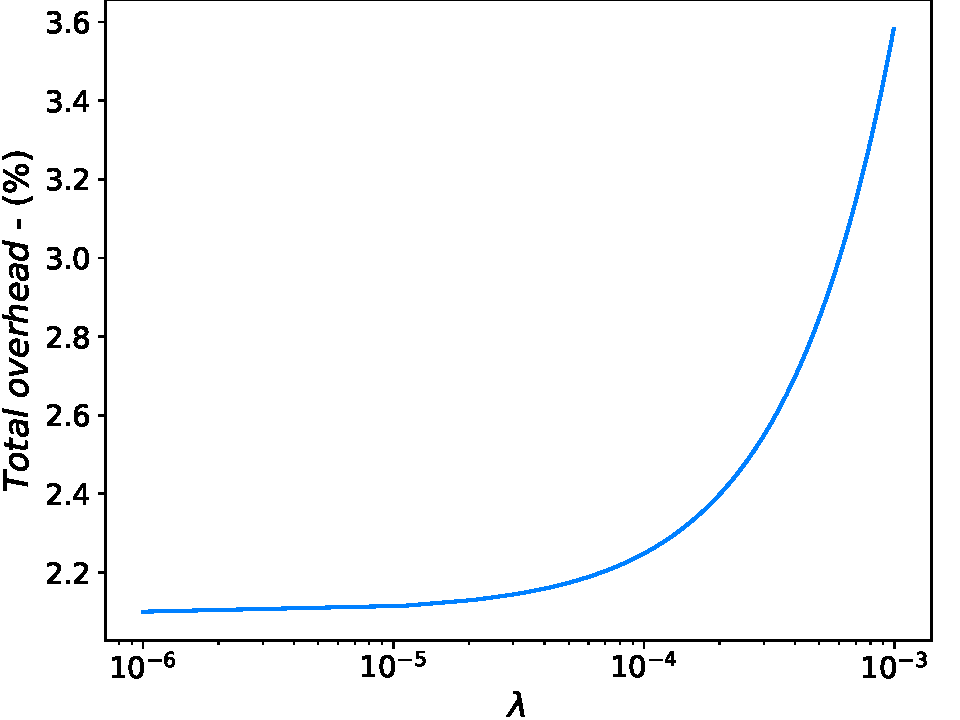
\includegraphics[width=0.49\textwidth]{real_perc_tot_ovhd_SP_C.pdf} }}
    \subfloat[\centering \textbf{(b)} Problem size class D - $k=0.2$.]{{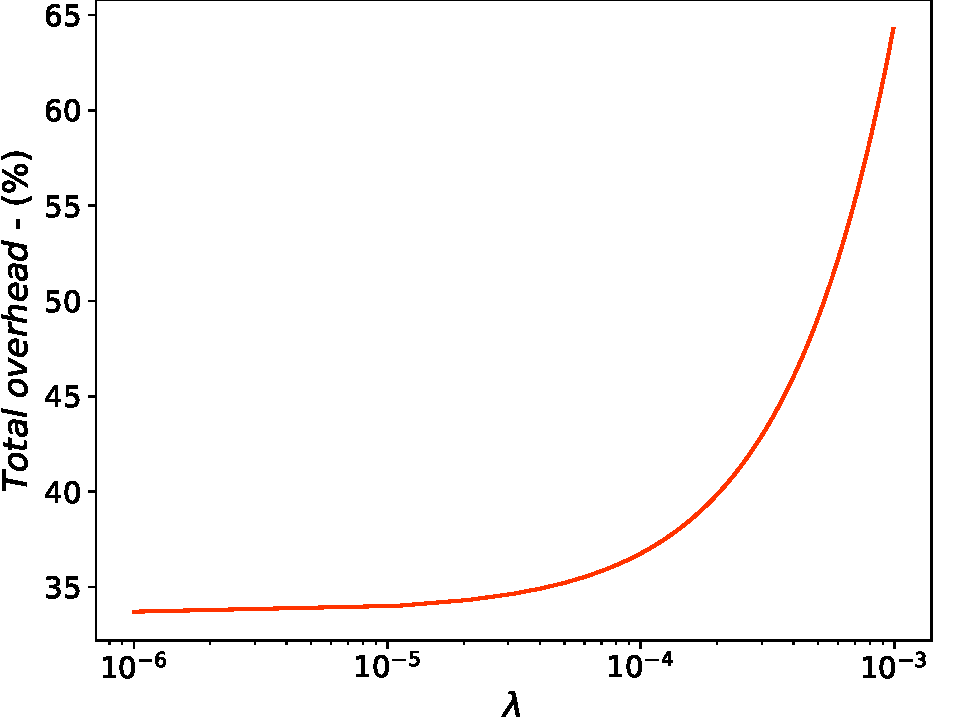
\includegraphics[width=0.49\textwidth]{real_perc_tot_ovhd_SP_D.pdf} }}}
    \caption{Percentage overhead caused by the sum of checkpointing time and time to recover from a failure, varying $\lambda$, on the execution of the sole application code.}%
    \label{fig:real_perc}%
\end{figure}}

From the above mentioned plots, it is possible to notice that, as expected, although it is possible to bound the overhead caused by the performing of the checkpoints, in the case of a reliability critical system, the overhead caused by failures might highly endanger the performance of the execution anyways. More specifically, Figure~\ref{fig:real_perc}(a) shows how, on one hand, for smaller problem sizes, hence shorter execution and checkpoint times, the percentage overhead, including the time to recover from a failure, does not exceeds \emph{significantly} in absolute value the upper bound set for the application. In this case, an overhead of 2\% was tolerated, and, in a highly unreliable system, a maximum of cumulative 3.6\% overhead is registered. On the other hand, for bigger problem sizes, Figure~\ref{fig:real_perc}(b), setting an upper bound of 20\% on the overhead, while the trend is about the same, a higher failure rate significantly impacts on the performance, getting close to the the 65\% of the application code execution time, in the case of SP benchmark. The choice of a higher upper bound in the case of bigger problem sizes has been determined by a matter of common sense: with a value as small as the one provided for class C problem sizes, given the extended $T_{chk\_mean}$ and $T_{exc\_tot}$ of class D, the number of checkpoints completed at the end of the execution of the application would have been too few for a realistic HPC use case.

To generalize these results, we carried out some computation on our measurement, in order to evaluate the just mentioned results for a wider range of reasonable values of $k$. Exploiting the fact that real checkpoint and period times can be easily approximated by their mean, we estimated the results commented above, using different values of $k$. 

For construction of the \emph{Dynamic Checkpoint Rate Tuning}, we know that:
\begin{align}
    n*T_{chk\_mean} &= k*n*(T_{period} - T_{chk\_mean})\label{eq:extract}\\
    T_{chk\_mean} &= k*(T_{period} - T_{chk\_mean})\\
    (k+1)*T_{chk\_mean} &= k*T_{period}\\
    T_{period} &= \frac{(k+1)}{k}*T_{chk\_mean}\label{eq:period}
\end{align}

Moreover, in light of the result obtained in Equation~\ref{eq:period} and reminding that:
\begin{align}
    T_{exc\_tot} = n*(T_{period} - T_{chk\_mean})
\end{align}
where $T_{exc\_tot}$ is known, we can also extract $n$ as follows:
\begin{align}
    T_{exc\_tot} &= n*\left(\frac{(k+1)}{k}*T_{chk\_mean} - T_{chk\_mean}\right)\\
    \noalign{\vskip9pt}
    T_{exc\_tot} &= n * \frac{T_{chk\_mean}}{k}\\
    \noalign{\vskip9pt}
    n &= k * \frac{T_{exc\_tot}}{T_{chk\_mean}}
\end{align}

Figures~\multiref{fig:comp_c}{fig:comp_perc} show the same measurements of Figures~\multiref{fig:real_c}{fig:real_perc} for a wide range of reasonable values of $k$.

Confirming the expectations given by the previous plots, we can observe that, although lower values of $k$ lead to higher values of $T_{failure}$, they are nonetheless suggested for smaller sized applications, since diminishing the overhead caused by the time spent re-executing lost computation, does not entails a smaller overhead, not even in a reliability critical system, such as the one characterized by $\lambda=10^{-3}$. Conversely, a bigger problem size, combined to a higher failure rate, might lead to an inversion of this trend. Figures~\ref{fig:comp_d}(b)~and~\ref{fig:comp_perc}(b) show how, with lower values of $k$, not only the total overhead significantly grows with the growing of $T_{failure}$, but also, for values of $\lambda$ \emph{high enough}, it might exceed the total overhead produced by a bigger $k$. More specifically, it is possible to see how, with $k=0.05$ (i.e. upper bound of 5\% in the checkpoint time overhead), while, in reliability safe systems, we measure a reasonably low overhead, around values of $\lambda=10^{-4}$, for all of the three benchmarks, it not only doubles its impact, but also exceeds the one produced by higher values of $k$. The conclusion of this evaluation is that, although, in reliable systems, the choice of the $k$ parameter is directly proportional to the amount of total overhead caused by both checkpoint time and time to recover from a failure, in systems where failures occurs with a higher frequency, the problem size is to consider in order not to lose the gain in specificity provided by the \emph{Dynamic Checkpoint Rate Tuning}. For this reason, a framework like BarbequeRTRM, in which the system state is constantly monitored and the checkpoint rate is tuned and adapted to each specific application, is an important resource for a better exploitation of HPC potentialities.

{\captionsetup[subfloat]{labelformat=empty}
\begin{figure}
    \centering
    {
    \subcaption[]{Benchmark: BT}
    \subfloat[\centering]{{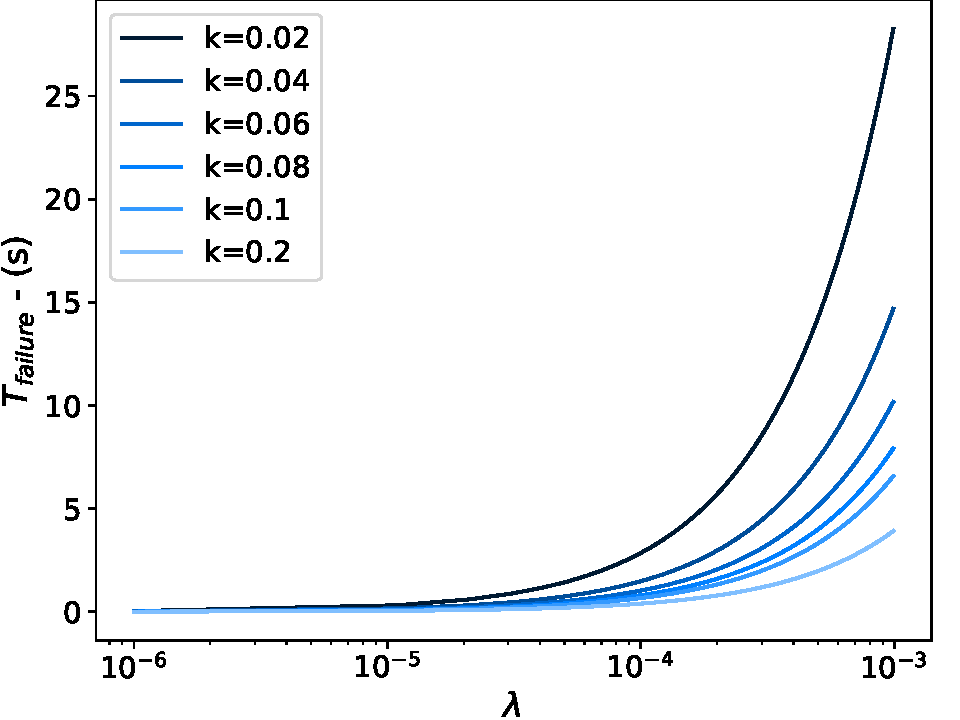
\includegraphics[width=0.49\textwidth]{avg_reset_time_BT_C.pdf} }}
    \subfloat[\centering]{{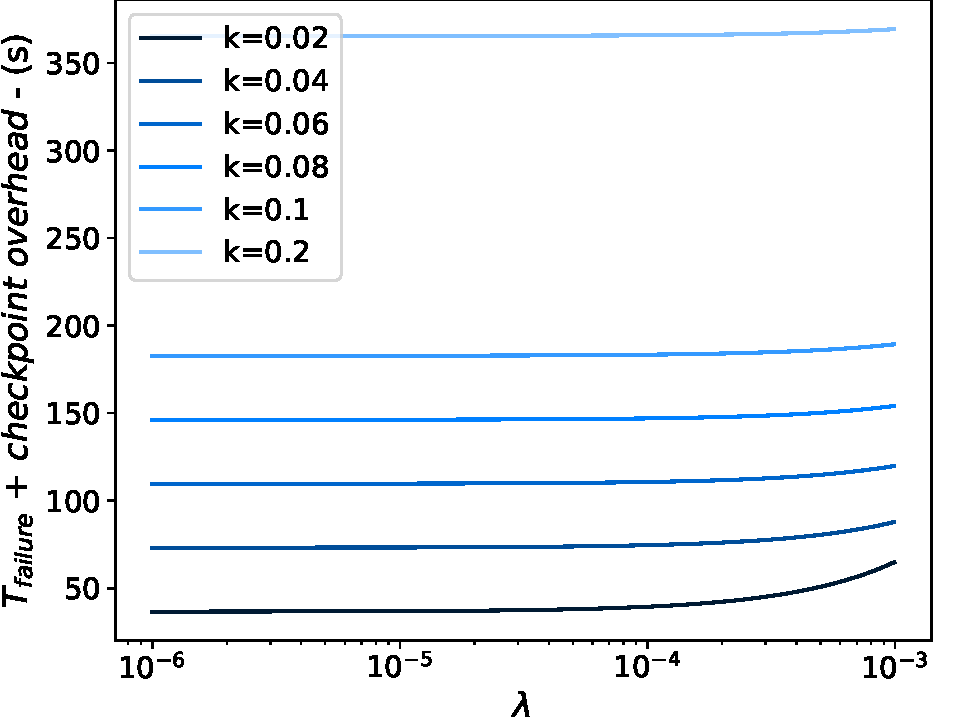
\includegraphics[width=0.49\textwidth]{avg_tot_ovhd_BT_C.pdf} }}\vspace{-1.1em}}
    {
    \subcaption[]{Benchmark: LU}
    \subfloat[\centering]{{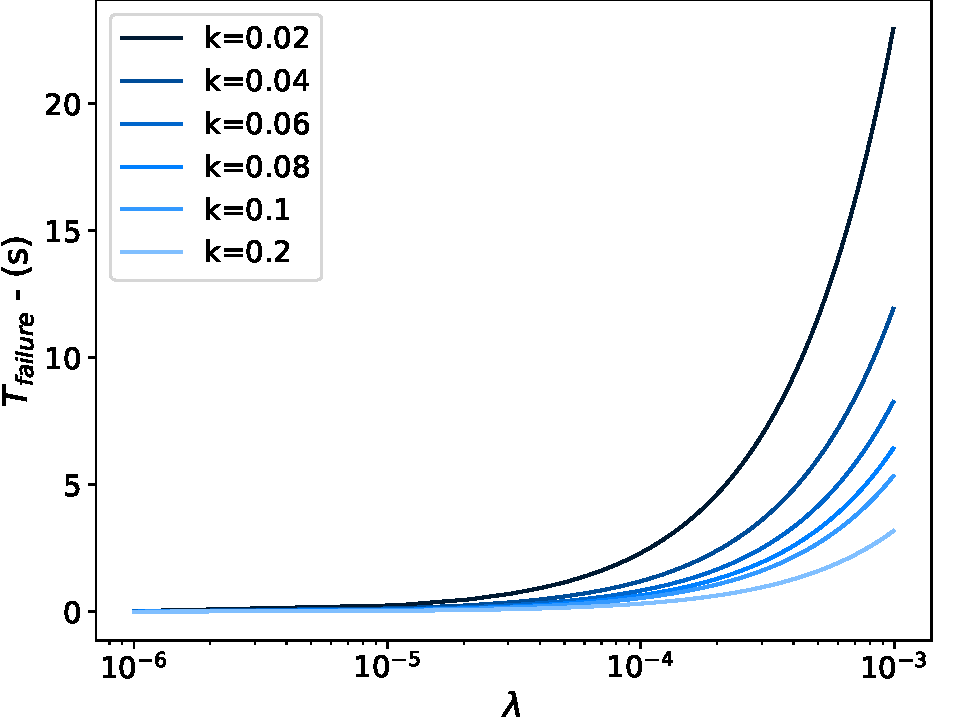
\includegraphics[width=0.49\textwidth]{avg_reset_time_LU_C.pdf} }}
    \subfloat[\centering]{{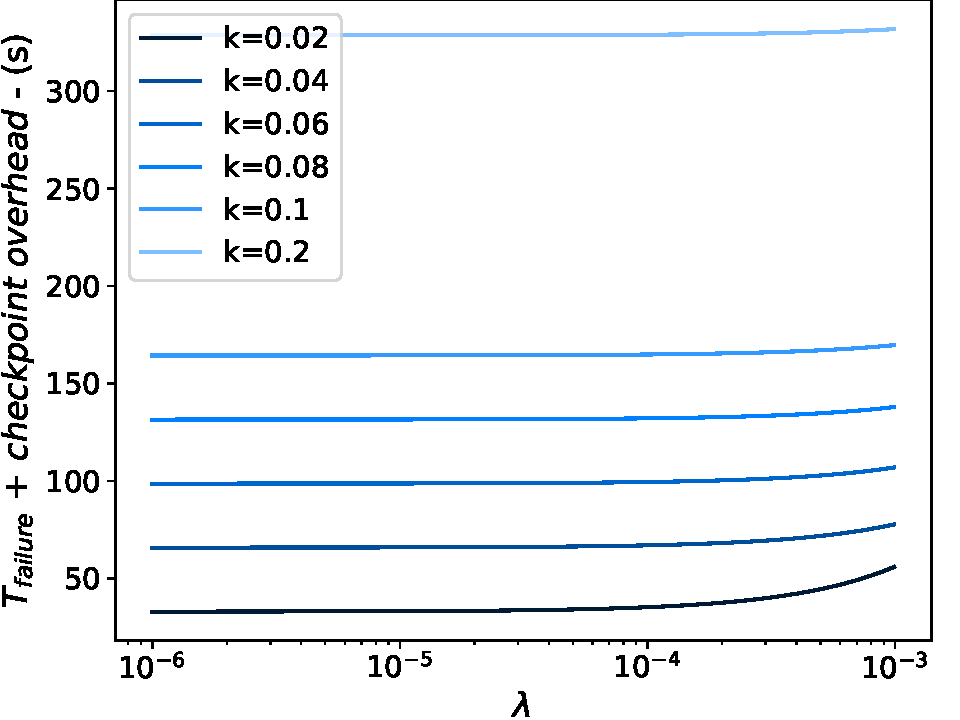
\includegraphics[width=0.49\textwidth]{avg_tot_ovhd_LU_C.pdf} }}\vspace{-1.1em}}
    {
    \subcaption[]{Benchmark: SP}
    \subfloat[\centering \textbf{(a)} Estimated mean overhead caused by the re-execution of application code in case of failure, varying $\lambda$ and $k$.]{{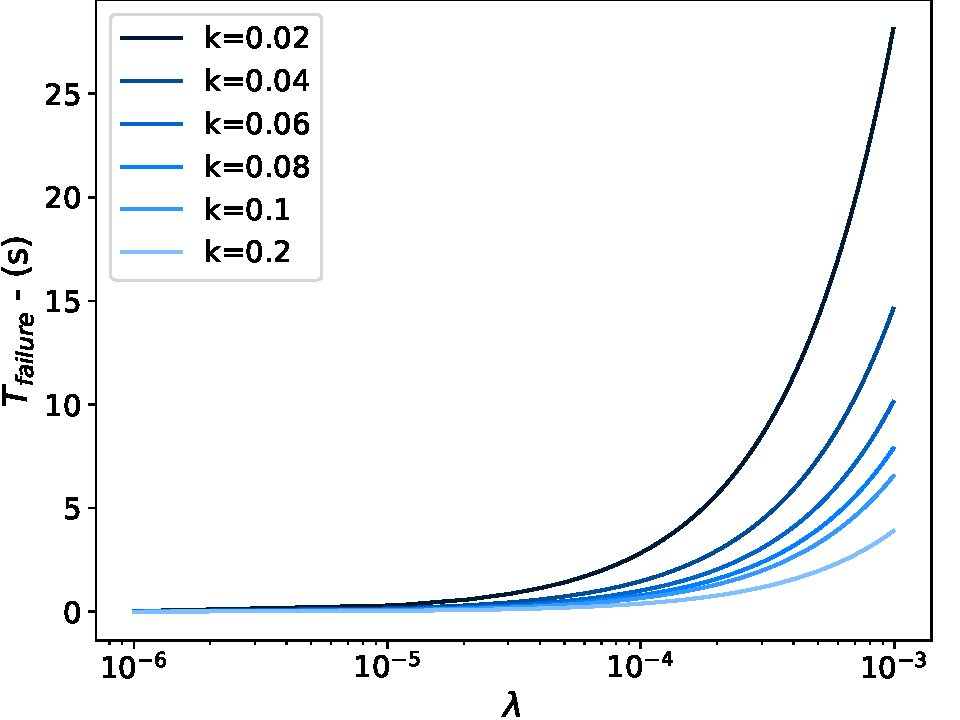
\includegraphics[width=0.49\textwidth]{avg_reset_time_SP_C.pdf} }}
    \subfloat[\centering \textbf{(b)} Sum of the value of \textbf{(a)} plus the checkpoint overhead, varying $\lambda$ and $k$.]{{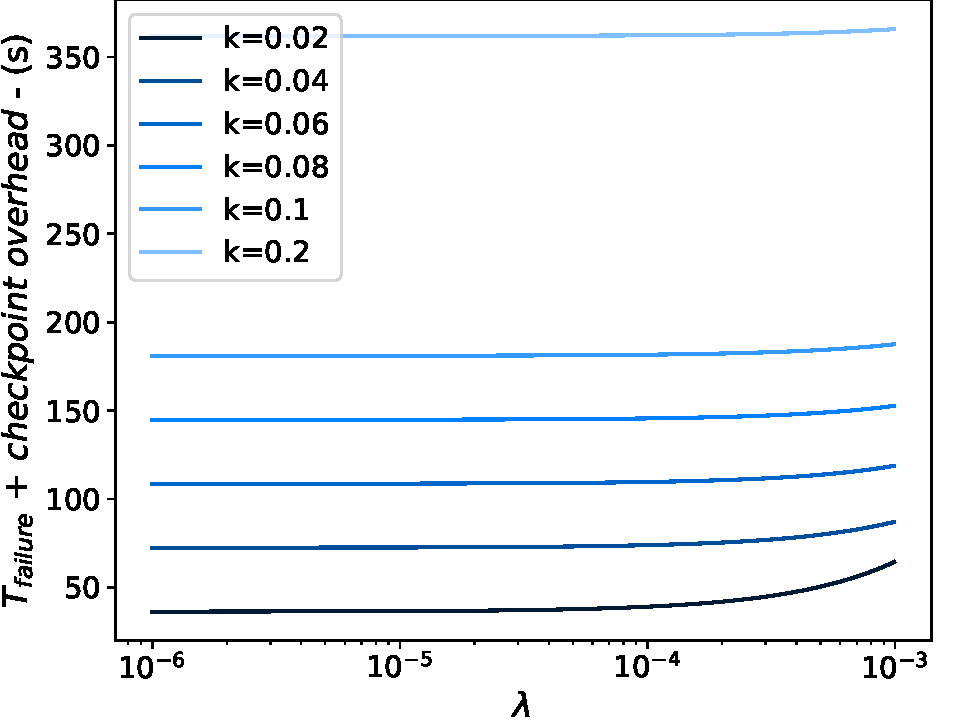
\includegraphics[width=0.49\textwidth]{avg_tot_ovhd_SP_C.pdf} }}}
    \caption{Plot of \textbf{(a)} $T_{failure}$, \textbf{(b)} $T_{failure}+checkpoint\ overhead$, varying $\lambda$ and $k$ - Problem size class C, estimate in seconds.}%
    \label{fig:comp_c}%
\end{figure}}

{\captionsetup[subfloat]{labelformat=empty}
\begin{figure}
    \centering
    {
    \subcaption[]{Benchmark: BT}
    \subfloat[\centering]{{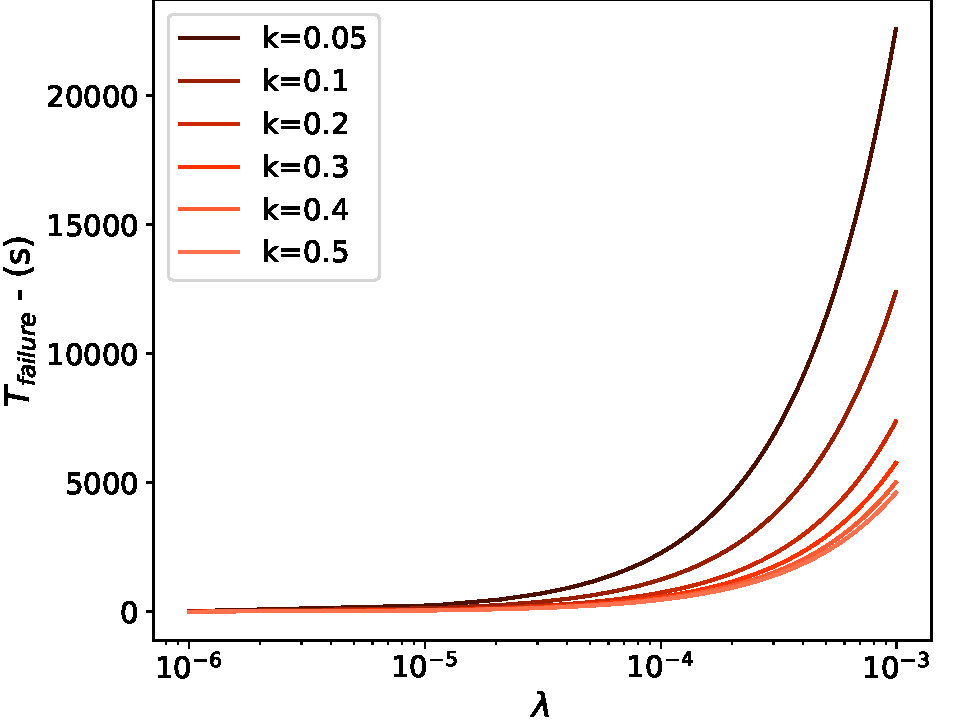
\includegraphics[width=0.49\textwidth]{avg_reset_time_BT_D.pdf} }}
    \subfloat[\centering]{{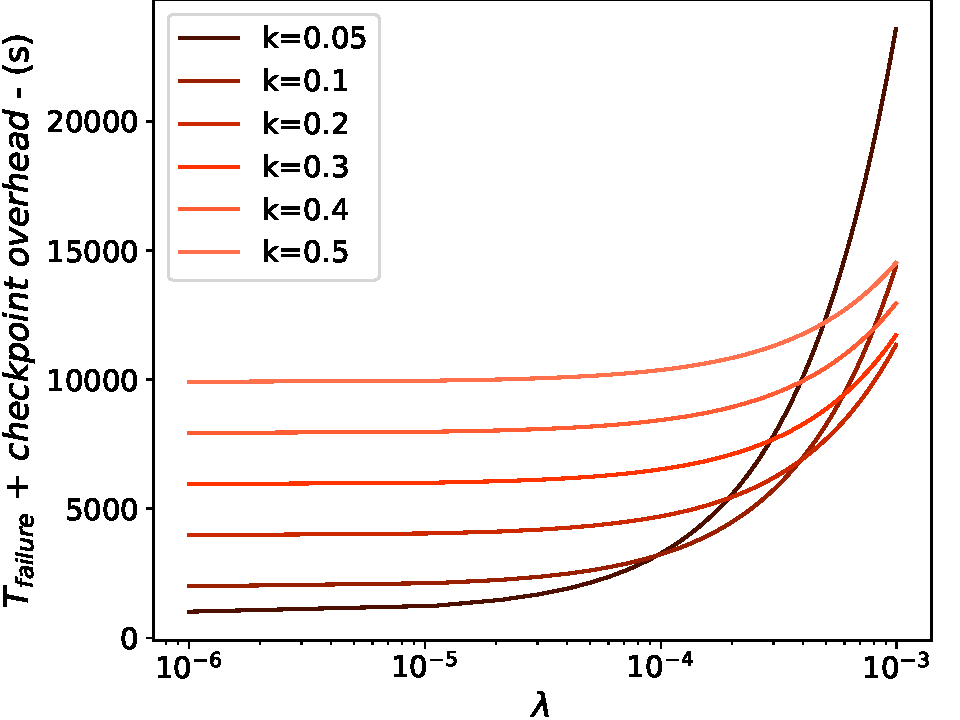
\includegraphics[width=0.49\textwidth]{avg_tot_ovhd_BT_D.pdf} }}\vspace{-1.1em}}
    {
    \subcaption[]{Benchmark: LU}
    \subfloat[\centering]{{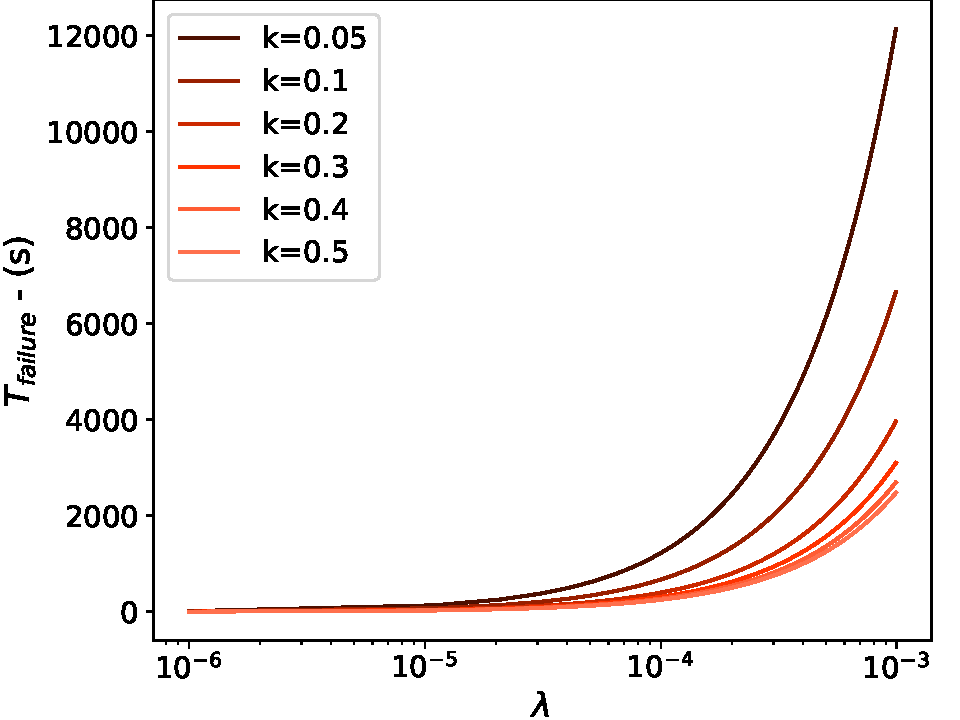
\includegraphics[width=0.49\textwidth]{avg_reset_time_LU_D.pdf} }}
    \subfloat[\centering]{{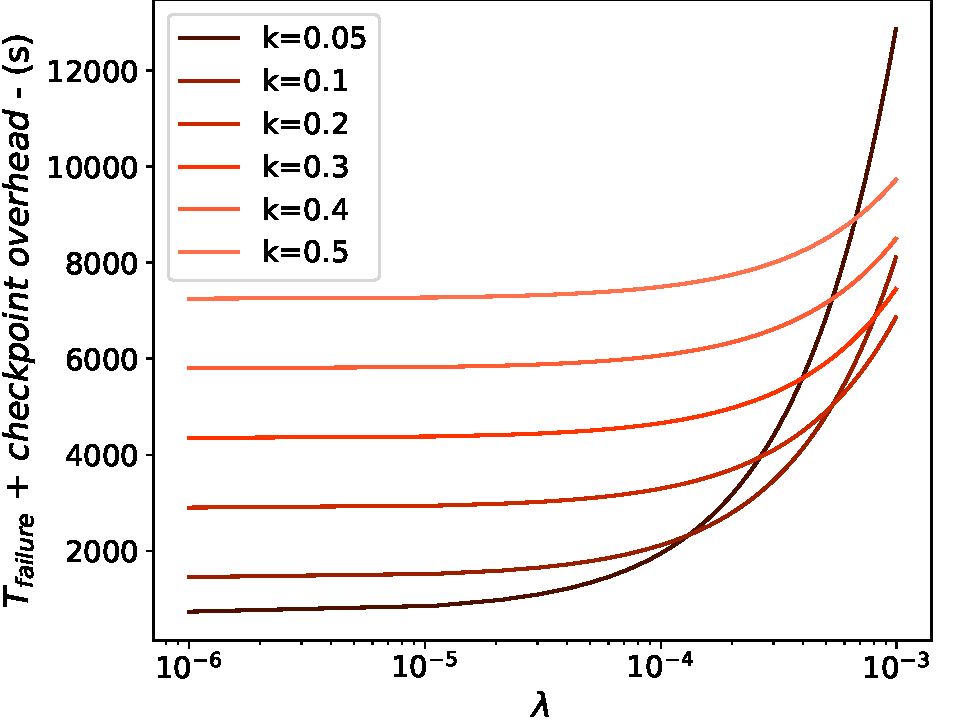
\includegraphics[width=0.49\textwidth]{avg_tot_ovhd_LU_D.pdf} }}\vspace{-1.1em}}
    {
    \subcaption[]{Benchmark: SP}
    \subfloat[\centering \textbf{(a)} Estimated mean overhead caused by the re-execution of application code in case of failure, varying $\lambda$ and $k$.]{{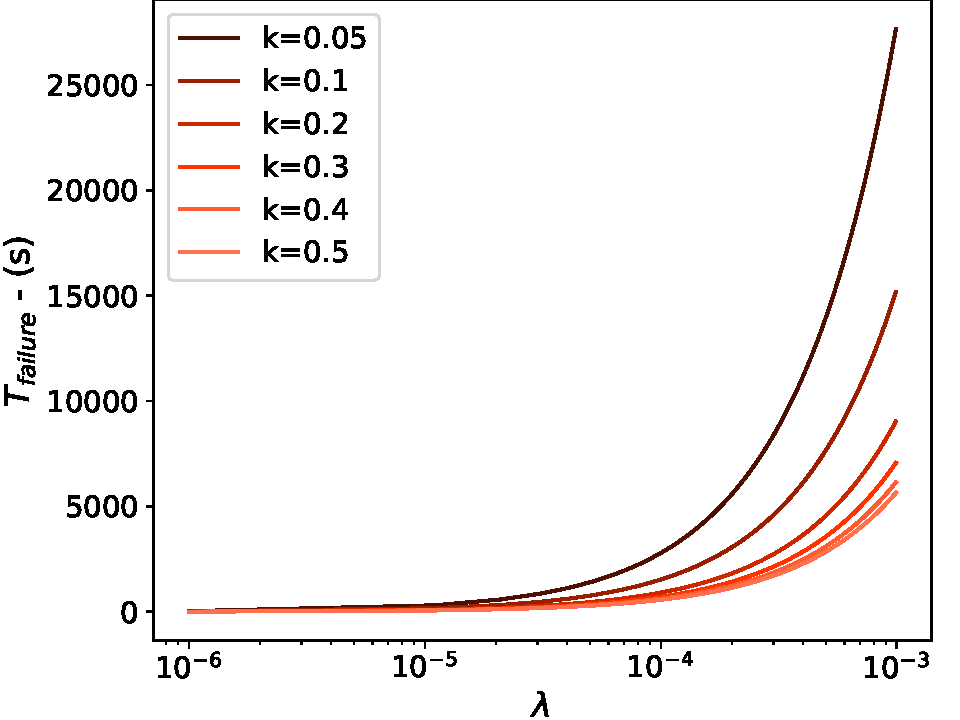
\includegraphics[width=0.49\textwidth]{avg_reset_time_SP_D.pdf} }}
    \subfloat[\centering \textbf{(b)} Sum of the value of \textbf{(a)} plus the checkpoint overhead, varying $\lambda$ and $k$.]{{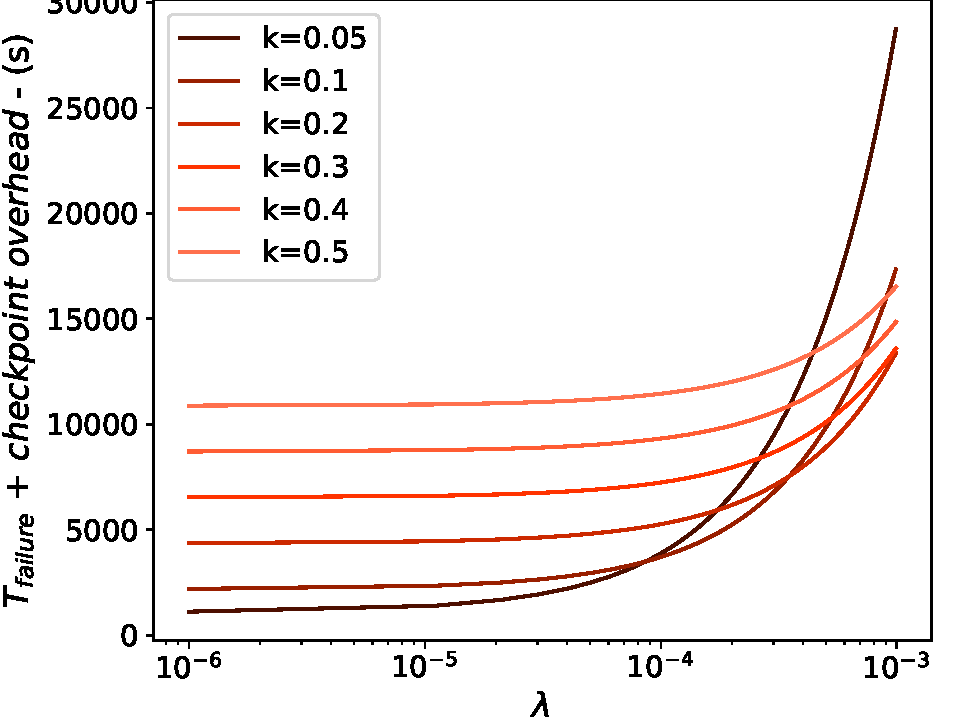
\includegraphics[width=0.49\textwidth]{avg_tot_ovhd_SP_D.pdf} }}}
    \caption{Plot of \textbf{(a)} $T_{failure}$, \textbf{(b)} $T_{failure}+checkpoint\ overhead$, varying $\lambda$ and $k$ - Problem size class D, estimate in seconds.}%
    \label{fig:comp_d}%
\end{figure}}

{\captionsetup[subfloat]{labelformat=empty}
\begin{figure}
    \centering
    {
    \subcaption[]{Benchmark: BT}
    \subfloat[\centering]{{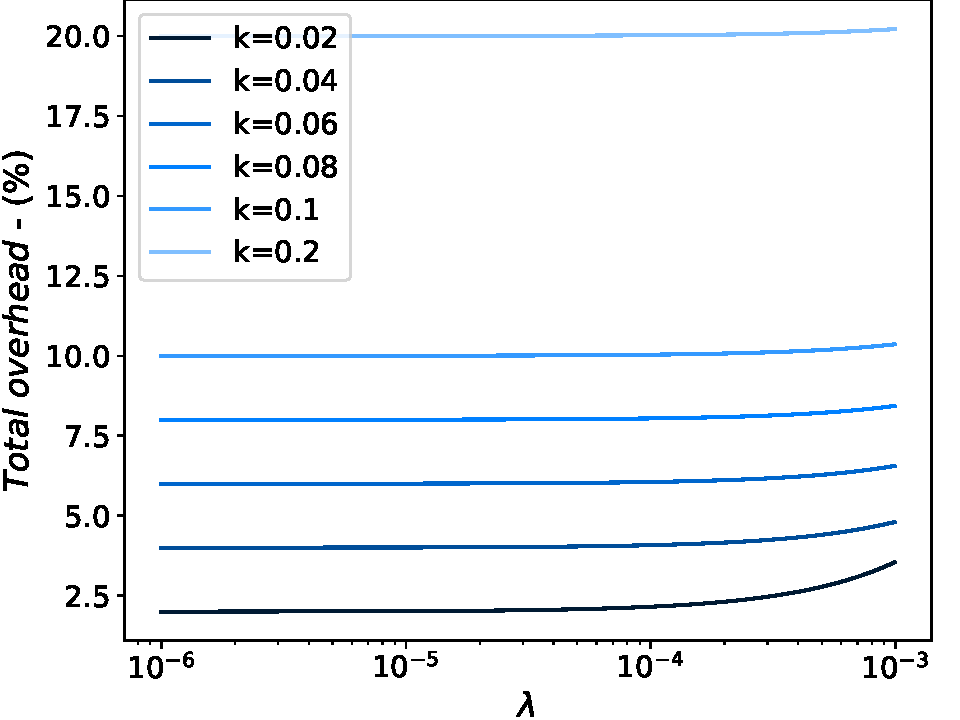
\includegraphics[width=0.49\textwidth]{perc_tot_ovhd_BT_C.pdf} }}
    \subfloat[\centering]{{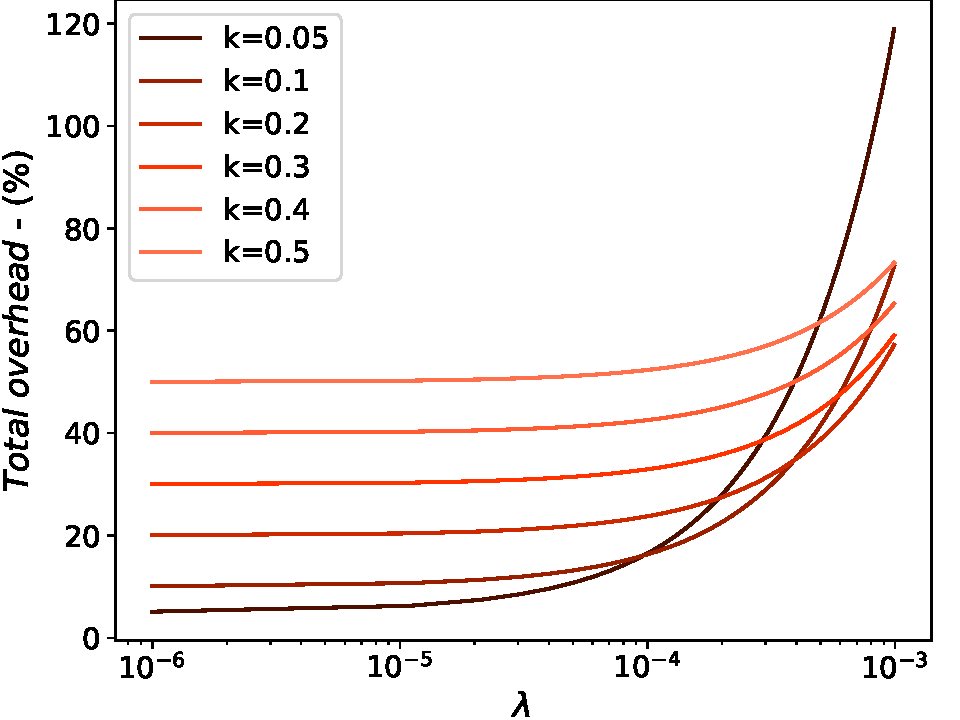
\includegraphics[width=0.49\textwidth]{perc_tot_ovhd_BT_D.pdf} }}\vspace{-1.1em}}
    {
    \subcaption[]{Benchmark: LU}
    \subfloat[\centering]{{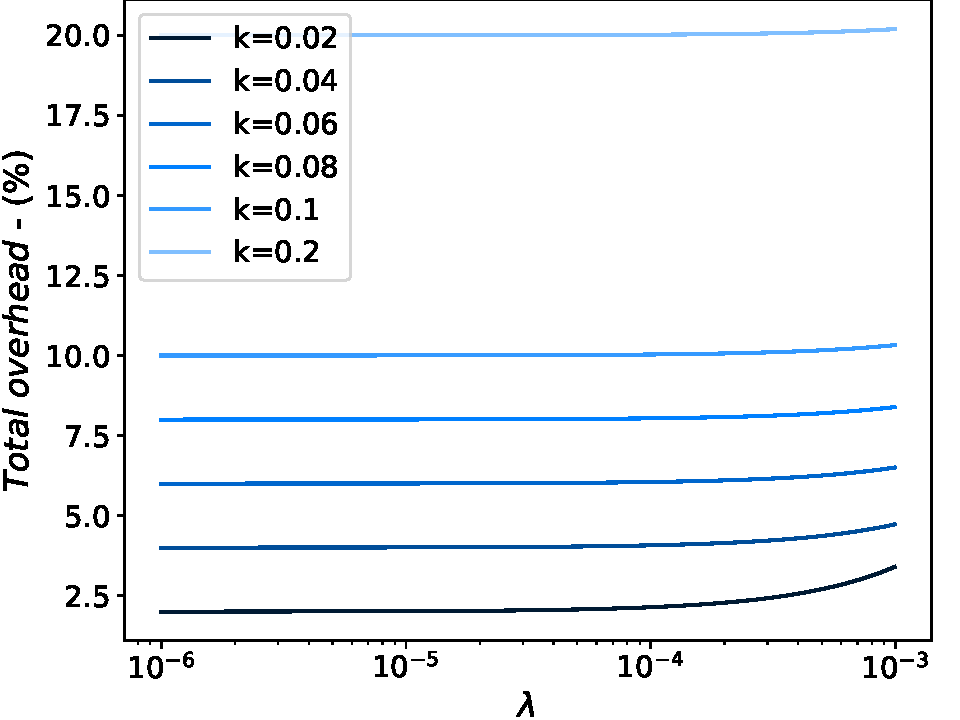
\includegraphics[width=0.49\textwidth]{perc_tot_ovhd_LU_C.pdf} }}
    \subfloat[\centering]{{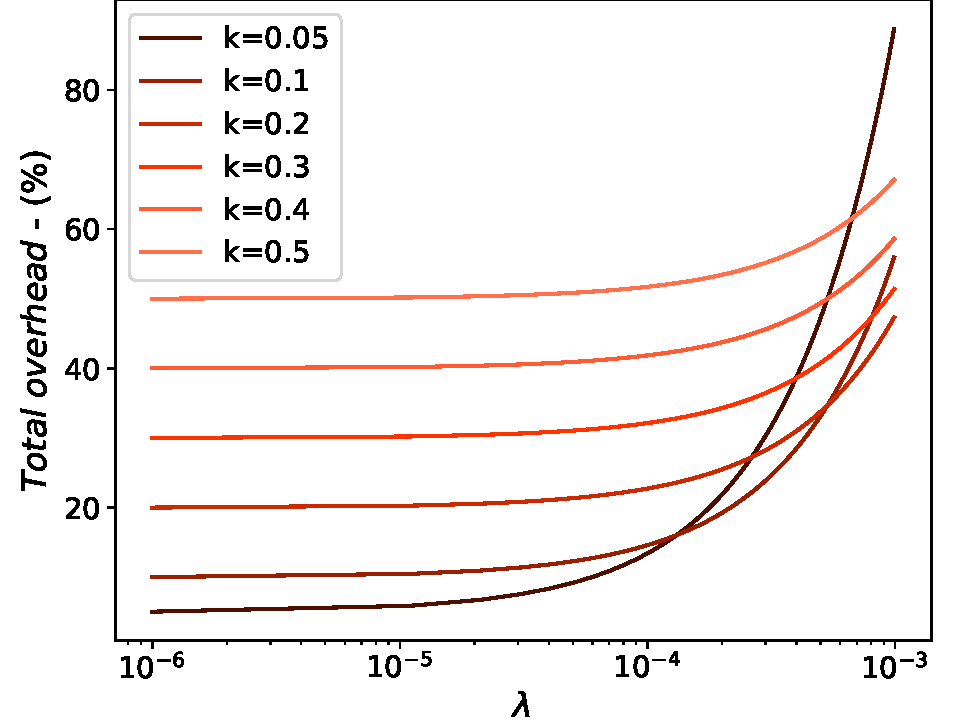
\includegraphics[width=0.49\textwidth]{perc_tot_ovhd_LU_D.pdf} }}\vspace{-1.1em}}
    {
    \subcaption[]{Benchmark: SP}
    \subfloat[\centering \textbf{(a)} Problem size class C.]{{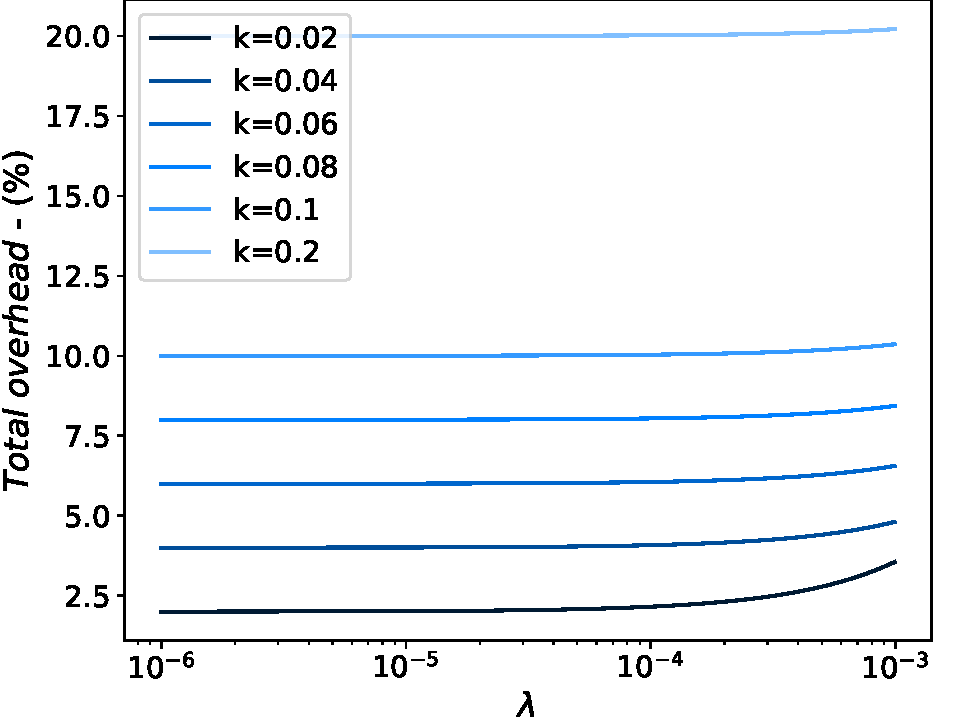
\includegraphics[width=0.49\textwidth]{perc_tot_ovhd_SP_C.pdf} }}
    \subfloat[\centering \textbf{(b)} Problem size class D.]{{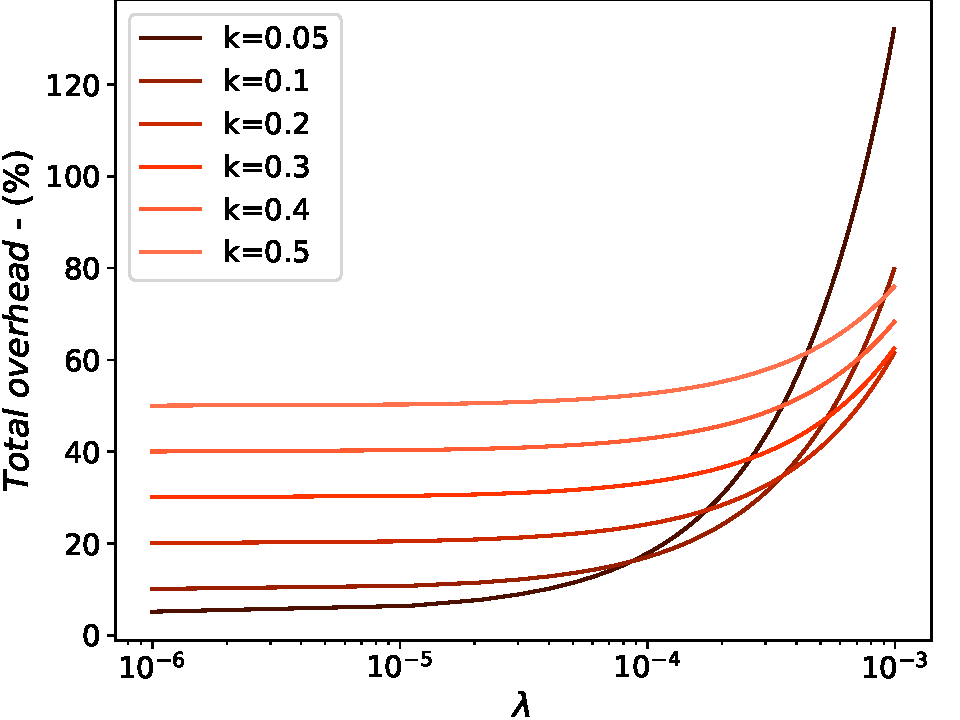
\includegraphics[width=0.49\textwidth]{perc_tot_ovhd_SP_D.pdf} }}}
    \caption{Estimated percentage overhead caused by the sum of checkpointing time and time to recover from a failure, varying $\lambda$, on the execution of the sole application code.}%
    \label{fig:comp_perc}%
\end{figure}}
\newpage
\section{Reliam Resource Allocation Policy}
As explained in Section~\ref{sec:poldesign}, the Reliam Resource Allocation Policy is composed by two main components: the mathematical model behind the CPU quota allocation, based on a modification of the PID controller model, and the selection of the CPU cores, based on reliability criteria. The first component aims to reduce the CPU utilization, in order to favor applications parallelization, while the second one has been designed to improve the reliability of the hardware components, minimizing their aging. Thanks to the low interdependence of the two components, it has been possible to test their objectives separately. The results of the first set of experiments will show the behavior of the controller, depending on the tuning of the controlling parameters. In such regard, three different use cases will be provided as a guideline in the setting of the policy. In the second set of tests, the effectiveness of the reliability decisions of the policy will be evaluated and commented. For this purpose, DCworms has been used in order to simulate a multi-core system.

\subsection{CPU quota allocation}
In this section the guidelines for tuning the modified PID controller model will be provided and the evaluation of its effectiveness  will take place, considering three different use cases of the CPU quota allocation mechanism.

\subsubsection{PID controller parametric tuning properties}
PID controllers are one of the most widely and successfully used controllers in a variety of industrial areas \cite{1638134}.

As introduced in Section~\ref{sec:poldesign}, the PID controller is designed as a \emph{negative feedback model}, relying on proportional, integral and derivative contributions, weighted by coefficients, respectively, $k_p,\ k_i, \text{ and } k_d$. In their combination, they contribute to the control action $u$, as shown in the following expression:
\begin{align*}
u(t) = k_p\,\epsilon(t) + k_i\int\epsilon(t)\,dt + k_d\,\frac{d\,\epsilon(t)}{dt}    
\end{align*}
where $\epsilon(t)$ represents the error at time $t$.

In order to properly tune a PID controller, we need to focus on four of its properties \cite{zhong2006pid}:
\begin{description}
\item[Rise Time:] time taken for the output to rise beyond 90\% of the desired level for the first time.
\item[Overshoot:] how much the the peak level is higher than the steady state, normalized against the steady state.
\item[Settling Time:] time taken for the system to converge to its steady state.
\item[Steady-State Error:] difference between the steady-state output and the desired output.
\end{description}

The increasing of each of the controller coefficients, $k_p,\ k_i, \text{ and } k_d$ has a different effect on each of the above mentioned properties. A summary of such effect is provided by Table~\ref{tab:pideffect}.

\begin{table}[t]
    \centering
    \begin{tabular}{|c||c|c|c|c|}
        \cline{2-5}
         \multicolumn{1}{l||}{}& \emph{Rise Time} & \emph{Overshoot} & \emph{Settling Time} & \emph{S-S Error}\\
        \hline\hline
        $k_{p}$ & Decrease & Increase & - & Decrease\\
        $k_{i}$ & Decrease & Increase & Increase & Eliminate\\
        $k_{d}$ & - & Decrease & Decrease & - \\
        \hline
    \end{tabular}
    \caption{Effect of the increasing of the controller parameters on the PID properties \cite{zhong2006pid}.}
    \label{tab:pideffect}
\end{table}

\subsubsection{The modified PID controller}
As deeply examined in Section~\ref{sec:poldesign}, in this work we made some changes to the PID controller in order for it to better fit the resource allocation problem.

In the following, the reached CPU quota assignment model is summarized:

\begin{enumerate}[label=-]
    \item Control variable: $cv$
    \item Process variable: $\Delta$
    \item Setpoint: $\overline{\Delta}$
    \item Error: $\epsilon$
\end{enumerate}
where:
\begin{align*}
    \renewcommand{\arraystretch}{3}
    \begin{array}{ll}
        cv &= 
        \begin{cases}
                k_{p}*\epsilon_r + k_{i}*\sum_{k\in R}\epsilon_{k} + k_d*(\epsilon_{r}-\epsilon_{r-1}) & \qquad \mbox{if } \epsilon\neq 0 \\
        	    0 & \qquad\mbox{otherwise} 
        \end{cases}\\
        \Delta &= 
            \begin{cases}
        	    CPU_{A} - CPU_{U} \hfill& \qquad \mbox{if } CPU_{A} > CPU_{U} \\
        	    \Delta_{NEG} &\qquad \text{otherwise}
    	    \end{cases}\\
    	    \epsilon &=
    	    \begin{cases}
        	    \overline{\Delta} - \Delta &\qquad\mbox{if } |\overline{\Delta}-\Delta| \geq \overline{\Delta}\mbox{}\\
        	    0 &\qquad \mbox{otherwise}
    	    \end{cases}
	\end{array}
\end{align*}

In our model, the proportional, integral and derivative coefficients, respectively, $k_p,\ k_i, \text{ and } k_d$, need to be properly tuned taking into consideration the target application. The tuning of such parameters is highly dependent on the workload and the resource availability in the system, as much as on the priority assigned to each application and the degree of parallelization desired for the system.

Although the mathematical model presented by this work shows an essential difference with respect to the simple PID controller model, due to the resetting of the integral and derivative contributions in the case of $\epsilon=0$, the effects of the controlling coefficients summarized in Table~\ref{tab:pideffect} nonetheless apply. Nevertheless, some considerations need to be made. Since applications are usually limited in time and not always constant at steady state, in this application area the concept of Steady-State Error might not be significant and the contribution of $k_{i}$ might not lead to its elimination. Moreover, Rise Time highly depends on the initial CPU quota assignment $CPU_{A_{ini}}$ which might be a straight away overshooting, hence, it is significant only in the case of $CPU_{A_{ini}} < CPU_{U_{ideal}}$, where the second term is the desired output of the policy. Also Settling Time, in the presented implementation, acquires a slight different meaning. Since the controller contributions are reset every time $\epsilon=0$ and, in any case, a steady-state does not always exist due to the possible variable workload of the application, we will refer, with Settling Time, to the first time the output of the controller matches the set point.

As anticipated above, a \emph{unique} optimal tuning of the three parameters of the controller does not exist, since it depends on the objective tried to be reached. In the following, three reasonable scenarios will be considered:
\begin{description}
\item[Scenario 1: massively parallel system.] Consider a system with limited computational resources with respect to the amount of parallel application executing simultaneously: the occurrence of a significant overshooting for an application might result in a waste in performance for the others, constrained for no reason with a CPU quota lower than the required.
\item[Scenario 2: mixed application priority system.] Take into account a system characterized by a wide number of computational resources and a time constrained prioritized application running on it: in this case, overshooting would not represent a problem as big as an extended rising time. 
\item[Scenario 3: long lasting applications system.] Consider a long lasting application with recurring small variations in the workload: we might want that, when such fluctuations occur, the CPU quota adjusts accordingly, avoiding big overshooting and minimizing the settling time.
\end{description}

Given the considerations expressed above, an analysis regarding the variation of the controlling parameters results necessary in the use of the Reliam Resource Allocation Policy. For this reason, an experimental characterization of the three above mentioned scenarios will be provided and commented.

For the experimental evaluation of the CPU quota allocation of the Reliam Resource Allocation Policy, we chose the PARSEC benchmark \emph{Fluidanimate} launched with two threads, set $\Delta_{NEG}=25$, $\overline{\Delta}=5$ and the invocation period of the policy to 4 seconds. We performed our experiments knowing that the CPU usage of the application at issue is approximately $CPU_{U}= 200$.

\begin{figure}[t]
    \centering
    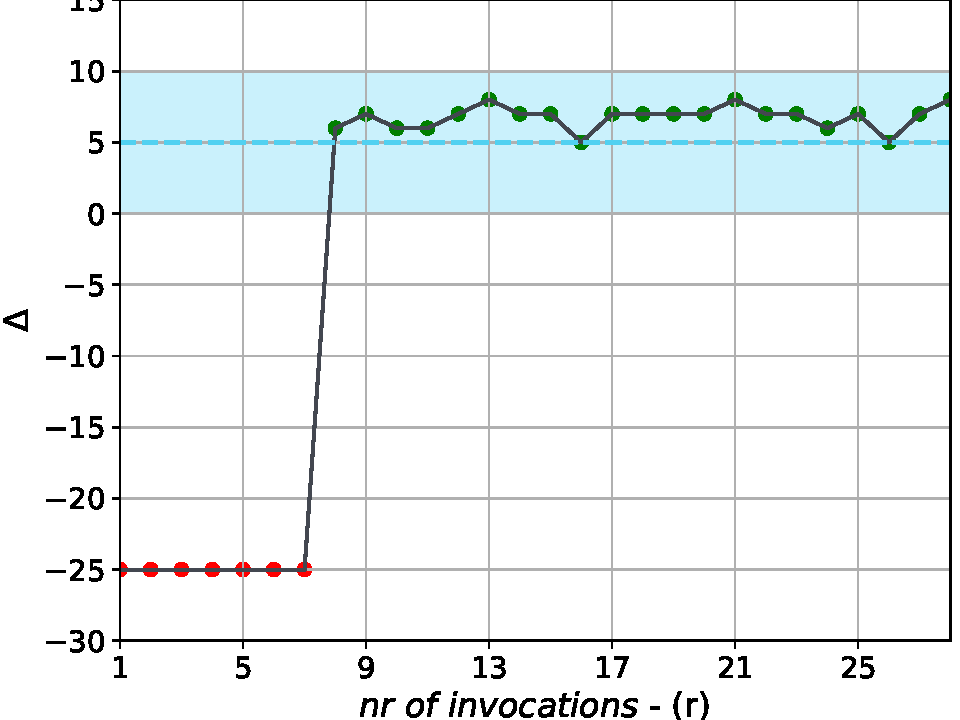
\includegraphics[width=0.8\textwidth]{delta_kp=0.5_ki=0_kd=0_def=100.pdf}
    \caption{\emph{Scenario 1}. Observed $\Delta$ at each invocation $r$ of the Reliam Resource Allocation Policy, setting $k_{p}=0.5\text{ and }k_{i}=k_{d}=0.0$. The blue area corresponds to the values of $\Delta$ such that $\epsilon=0$, the dashed line to $\overline{\Delta}$.}
    \label{fig:pid500}
\end{figure}

To match \textbf{Scenario 1}, we firstly consider an initial assigned CPU quota $CPU_{A_{ini}}=100$, since it is reasonable that an initial underestimation of the quota assignment is preferred in such conditions. To reach the objective, we set the controller up as purely proportional, i.e. eliminating the integral and derivative contributions. We expect from this settings a low\footnote{Lower than half of the absolute value of $\Delta_{NEG}$} or non-existent overshooting, due to the absence of the integral contribution.

We set the parameters as follows:
\begin{align*}
    k_p = 0.5 \quad k_i = 0.0 \quad k_d = 0.0
\end{align*}

The plot of the observed value of $\Delta$ at each invocation $r$ of the policy is shown in Figure~\ref{fig:pid500}. The underestimation of the CPU quota assignment is visible from the plot in the initial points, highlighted in red to be distinguished from the ones in green, producing $\epsilon=0$, hence, a correct assignment of the CPU quota. Those points correspond to the invocations of the policy in which the application uses all of the assigned resources, thus, an under-assignment is assumed and the value of $\Delta$ is approximated to $\Delta_{NEG}$ for a balanced functioning of the controller.

From the above mentioned Figure, it is possible to extract information about the PID properties discussed above.

As expected, no overshooting is present in the output of the controller, whose rising time, coinciding with the settling time, equals 8 invocations of the policy. In this scenario, no needless loss in terms of resource allocation is caused to other parallel applications, at the expenses of an initial under allocation for the one at issue. This approach favors the minimization of CPU utilization.

Starting from the previous settings, we consider a context more similar to \textbf{Scenario 2}. In this case, it is of greater importance to provide the application at issue with the needed CPU quota as soon as possible. Following the guidelines of Table~\ref{tab:pideffect}, we increase the value of $k_i$ leaving the other two coefficients unchanged.

The new setting becomes:
\begin{align*}
    k_p = 0.5 \quad k_i = 0.3 \quad k_d = 0.0
\end{align*}

The results of this configuration are shown in Figure~\ref{fig:pid530}.
As in the previous scenario, we identify the underestimation of the CPU quota in the initial points of the plot, characterized by $\Delta=\Delta_{NEG}$. Differently from before, at the fourth invocation, we observe a positive value of $\Delta$, exceeding the admissible range, represented by the blue area. Such points correspond to an over-assignment of CPU quota, hence, to real values of $\Delta$, which does not need to be approximated with $\Delta_{NEG}$ anymore. From Figure~\ref{fig:pid530}, we can observe a large overshooting, which distances $\Delta$ from the setpoint of 45 units. Although the settling time corresponds with the ninth invocations of the policy, the application have at its disposal all the needed resources already at invocation 4. This approach favors the prioritization of the resource assignment for the application at issue, which is provided with an overestimation of its expected usage. System-wide, this kind of approach might result in a possible deprivation of CPU quota for the applications parallel to the one at issue. In systems in which one main application needs to run with maximum priority with respect to the others, a configuration similar to the one just analyzed is to be considered for the former, while using an approach like the one described in Scenario~1 for the latters.
\begin{figure}[t]
    \centering
    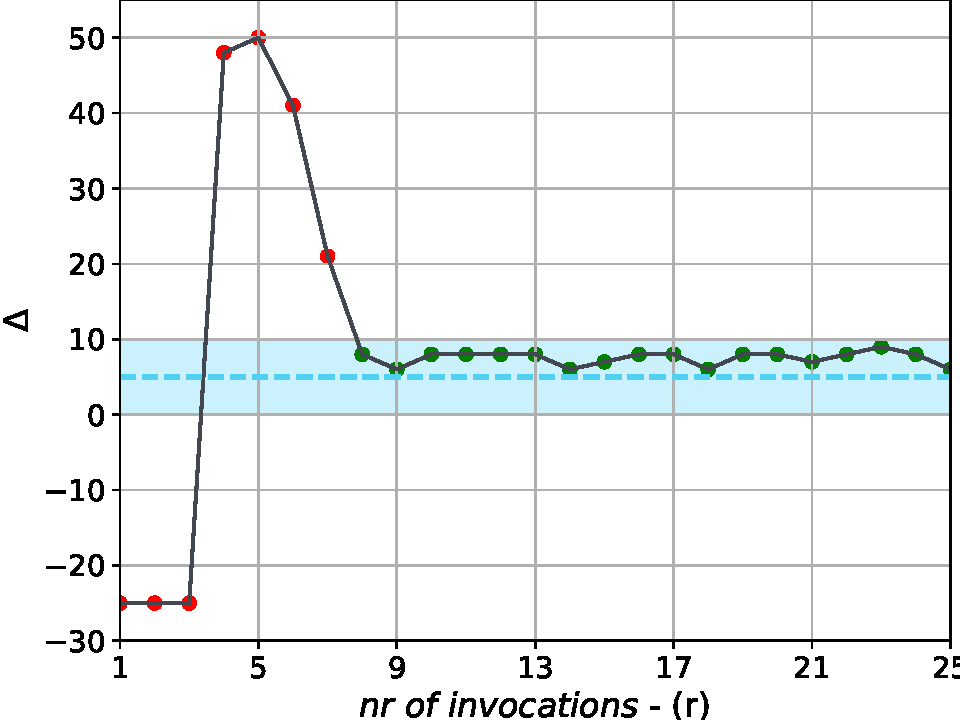
\includegraphics[width=0.8\textwidth]{delta_kp=0.5_ki=0.3_kd=0_def=100.pdf}
    \caption{\emph{Scenario 2}. Observed $\Delta$ at each invocation $r$ of the Reliam Resource Allocation Policy, setting $k_{p}=0.5\text{, }k_{i}=0.3\text{ and }k_{d}=0.0$. The blue area corresponds to the values of $\Delta$ such that $\epsilon=0$, the dashed line to $\overline{\Delta}$.}
    \label{fig:pid530}
\end{figure}

\begin{figure}[t]
    \centering
    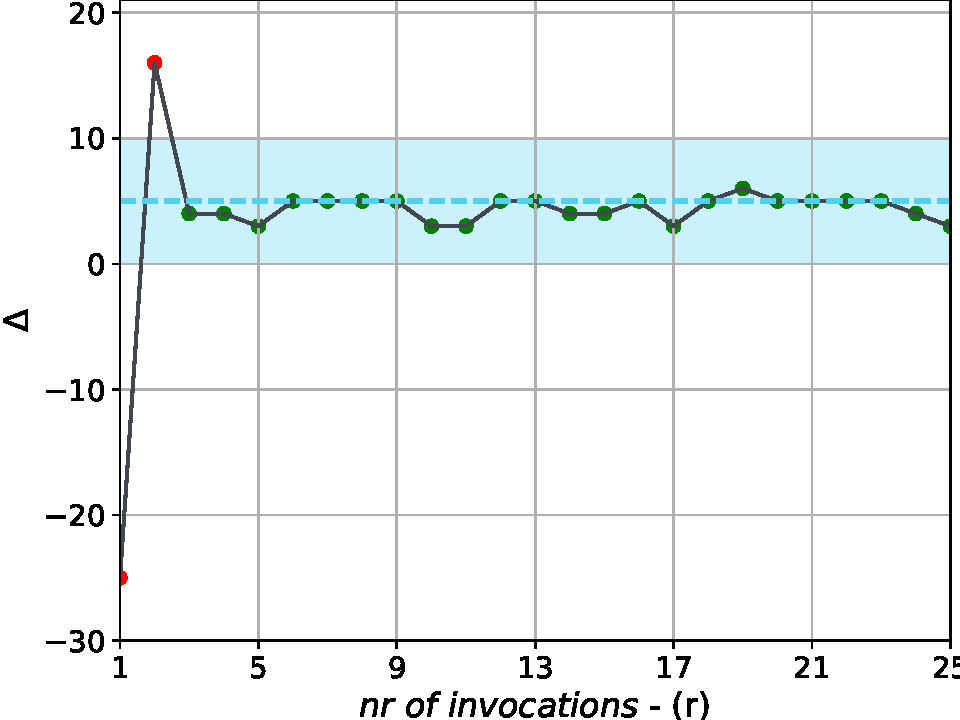
\includegraphics[width=0.8\textwidth]{delta_kp=0.3_ki=0_kd=0.3_def=200.pdf}
    \caption{\emph{Scenario 3}. Observed $\Delta$ at each invocation $r$ of the Reliam Resource Allocation Policy, setting $k_{p}=0.3\text{, }k_{i}=0.0\text{ and }k_{d}=0.3$. The blue area corresponds to the values of $\Delta$ such that $\epsilon=0$, the dashed line to $\overline{\Delta}$.}
    \label{fig:pid303}
\end{figure}

Finally, to simulate \textbf{Scenario 3}, we resorted to the characteristic differentiating our model from a simple PID controller: the resetting of the integral and derivative contributions each time the annulment of the error is reached. This property has the same effect of resetting the controller with a new $CPU_{A_{ini}}$, i.e. the value that has lastly guaranteed $\epsilon=0$. Since, in the case of a long lasting application, it is reasonable to consider as negligible the first settling time, we simulate the operating application providing to the controller $CPU_{A_{ini}}=200$, i.e. a value \emph{close enough} to the CPU quota our benchmark is able to use.

Following the guidelines provided by Table~\ref{tab:pideffect}, we lower $k_p$ and $k_i$ to lower Overshooting, and increased $k_d$ to decrease Settling Time.

The resulted settings lead to a PD controller with parameters:
\begin{align*}
    k_p = 0.5 \quad k_i = 0.0 \quad k_d = 0.3
\end{align*}

Figure~\ref{fig:pid303} shows the results of the last experiment. The low\footnote{With respect to the other scenarios.} under-estimation of the CPU quota allocation can be inferred from the speed at which $\Delta$ goes from negative to positive values. This transition happens in just one invocation: this verifies the closeness between $CPU_{A_{ini}}$ and the real CPU quota requirement of the application. As expected, the registered overshoot results low, just 11 units of $\Delta$, and settling time corresponds to just 3 invocations of the policy. 


\subsection{CPU cores selection}
This section will focus on the experiments performed on the \emph{Reliam Resource Allocation Policy} to test the effectiveness of the CPU cores selection.

As anticipated above, DCworms has been exploited to test the policy on a multi-node scale.

We set the environment in order to simulate a system composed of 4 nodes with 16 processors each, for a total of 64 CPUs. On this system we simulated the execution of 256 running tasks.

Moreover, we excluded from the simulation any kind of checkpointing backup, i.e. if a failure occurs in the processing element used by the application, it goes back to the start and performs again all the computation.

As explained in Section~\ref{sec:poldesign}, the \emph{Reliam Resource Allocation Policy} is able to make two kinds of reliability-aware decisions:
\begin{enumerate}[label={\arabic*)}]
    \item In the case of a non-full-loaded system, it delegates the execution of the running applications to the \emph{most reliable} cores, idling the left ones;
    \item In the case of an application bound solely to \emph{non-reliable} cores, it freezes the execution and migrates the application to \emph{more reliable} cores, if any.
\end{enumerate}

We neglected the simulation of the decision described in 1), due to the triviality of the evaluation of the effectiveness. If an application runs only on the most reliable cores, for construction, it minimizes the occurrence of failures, without providing any worsening to the reliability of the \emph{critical} cores.
Conversely, we evaluated the effectiveness of the decisions described in 2).

We simulated a workload almost saturating the computational resources, with a total execution time, in absence of failures, $T_{exc\_tot}$, equal to 200 invocations of the policy. We performed our experiments considering different failure rates. More specifically, we selected five different Mean Time Between Failure (MTBF), corresponding to a number of invocations such to verify the following equalities:
\begin{itemize}
    \item $\frac{T_{exc\_tot}}{MTBF}=4$
    \item $\frac{T_{exc\_tot}}{MTBF}=5$
    \item $\frac{T_{exc\_tot}}{MTBF}=6$
    \item $\frac{T_{exc\_tot}}{MTBF}=7$
    \item $\frac{T_{exc\_tot}}{MTBF}=8$
\end{itemize}

Moreover, we defined two criticality thresholds, as described in Section~\ref{sec:dcworms}. Firstly we set such threshold to 70\%. This setting implies for the policy to mark a processing unit as \emph{critical} when such \emph{criticality threshold} is reached.

\begin{figure}[t]
    \centering
    \subfloat[\centering Criticality threshold equal to 70\%. ]{{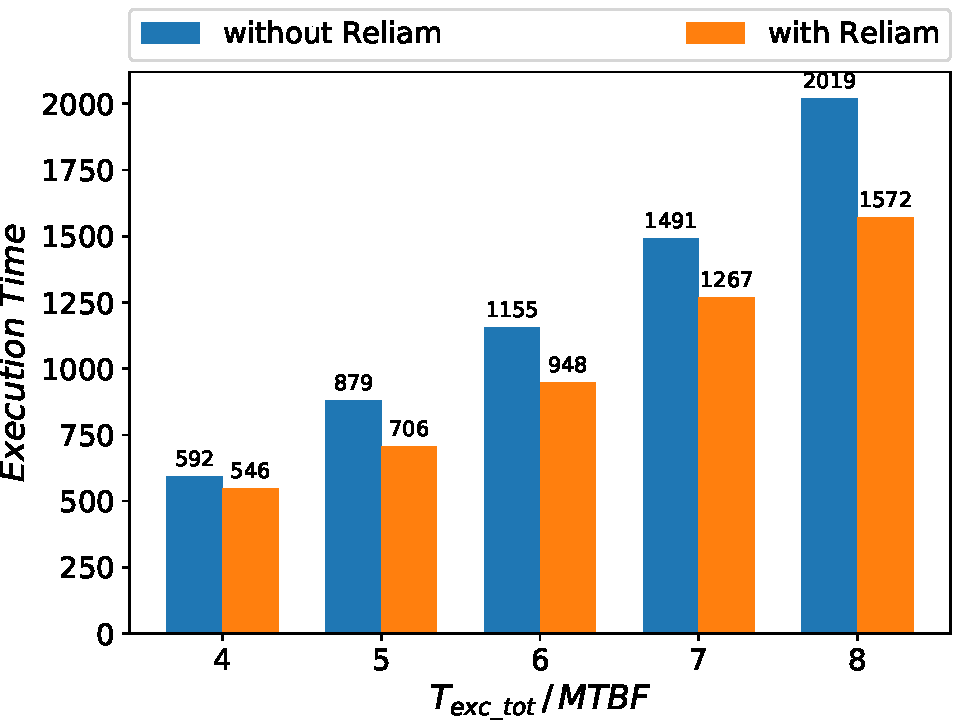
\includegraphics[width=0.55\textwidth]{exc_time_rel=70.pdf} }}
    \\\hspace{1em}
    \subfloat[\centering Criticality threshold equal to 80\%.]{{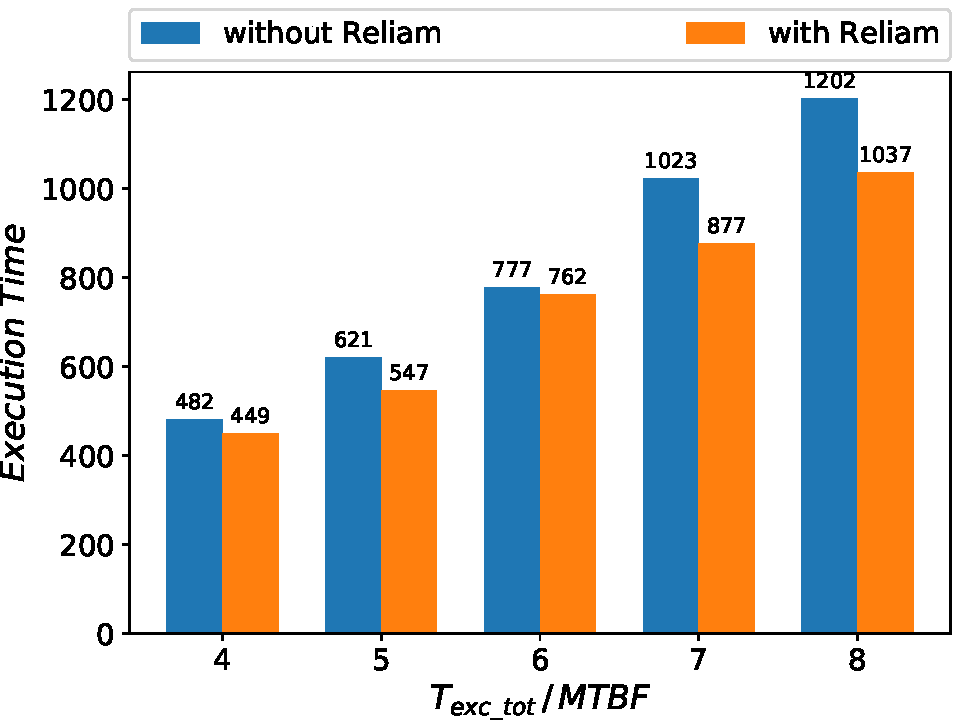
\includegraphics[width=0.55\textwidth]{exc_time_rel=80.pdf} }}
    \caption{Execution time (expressed in number of invocations) provided by basic policy (blue bars) and the Reliam Resource Allocation Policy (orange bars).}
    \label{fig:exc}%
\end{figure}

We collected data regarding execution time and peak temperature of the processors. Then we performed the same experiments moving the criticality threshold to 80\%. Figures~\multiref{fig:exc}{fig:af} show the data collected from the simulation of the workload using the \emph{Reliam Resource Allocation Policy}, comparing them to the ones extracted from the execution of the same workload using a simple policy, performing migration only in case of failure.

Figure~\ref{fig:exc} shows the execution time, expressed in number of invocations of the policy, obtained with and without the reliability decisions of the \emph{Reliam Resource Allocation Policy}. In both cases, characterized, respectively, by a criticality threshold equal to 70\% and to 80\%, we observed in a mitigation in the loss of performance proportional to the injected failure rate. Thanks to the reliability-aware decisions, the application have a bigger probability of not getting bound to cores considered more prone to failures, hence, the re-execution of the application code happens with a lower frequency, conferring, in the tested cases, a mitigation of the performance loss ranging between 8\% and and 22\% in the case of criticality threshold equal to 70\%, while between 7\% and 14\%, in the case of criticality threshold equal to 80\%.

\begin{figure}[t]
    \centering
    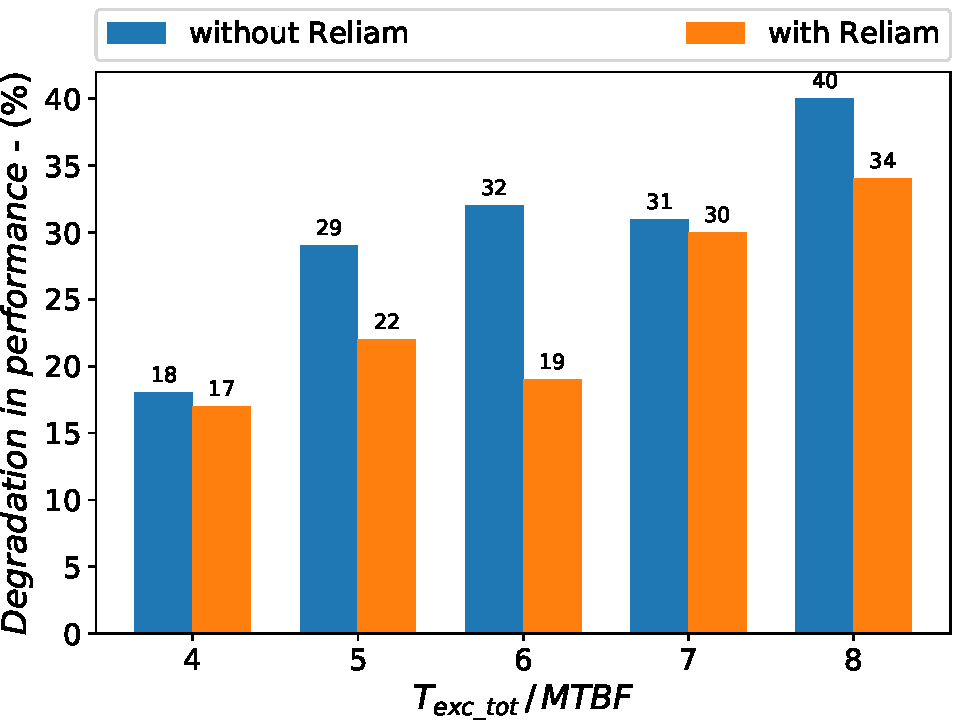
\includegraphics[width=0.8\textwidth]{degradation.pdf}
    \caption{Performance degradation between criticality thresholds 80\% and 70\% .}
    \label{fig:degradation}
\end{figure}

Another interesting insight provided by the tests is represented by the comparison of the two policies in the different reliability scenarios. In the case of criticality threshold equal to 70\%, the Reliam Resource Allocation Policy presents a lower degradation in terms of performance with respect to the 80\% case. In the best tested case, represented by $\frac{T_{exc\_tot}}{MTBF}=4$, the worsening in performance observed by comparing the execution time provided by each policy with the different criticality threshold is about the same (19\% without Reliam, 18\% using Reliam). For $\frac{T_{exc\_tot}}{MTBF}=8$, the results of the policy without reliability control in the case of criticality threshold equal to 70\% presented a worsening of the performance equal to the 40\% of the performances registered with criticality threshold equal to 80\%. Considering the same scenarios, introducing the reliability-aware decisions, we observe a worsening of only 34\%. Such results are summarized in Figure~\ref{fig:degradation}.


\begin{figure}[t]
    \centering
    \subfloat[\centering Criticality threshold equal to 70\%.]{{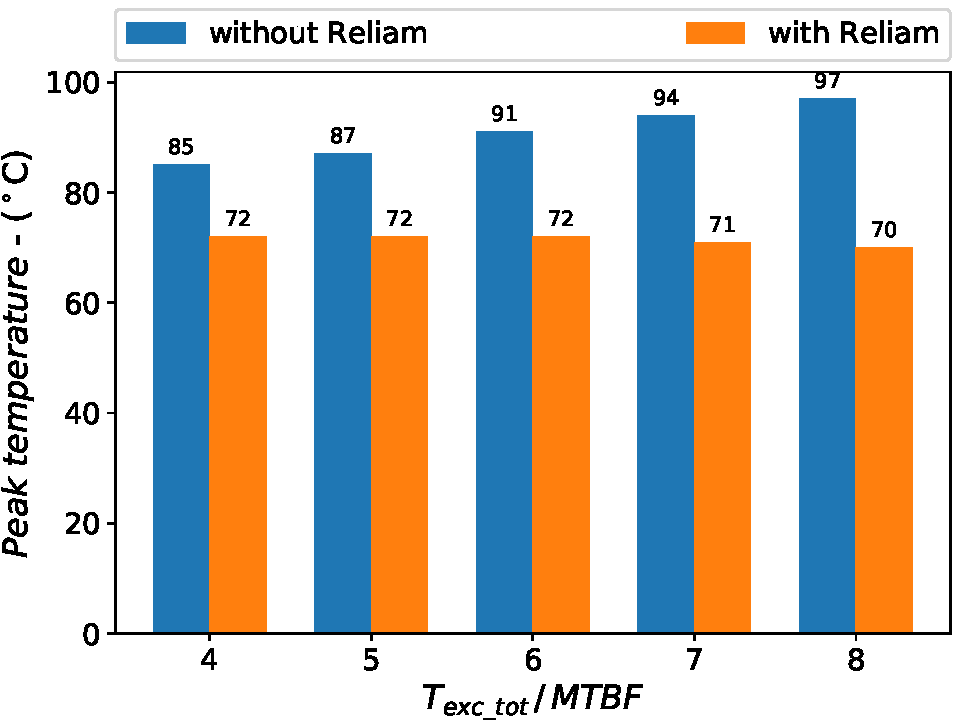
\includegraphics[width=0.5\textwidth]{peak_temp_rel=70.pdf} }}
    %\\\vspace{1em}
    \subfloat[\centering Criticality threshold equal to 80\%.]{{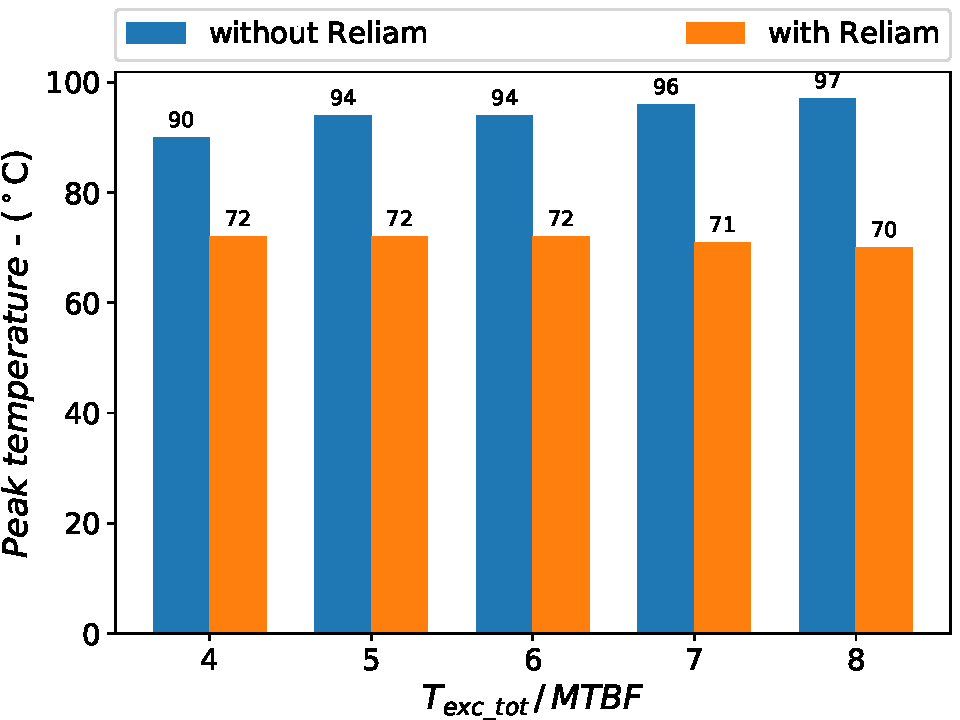
\includegraphics[width=0.5\textwidth]{peak_temp_rel=80.pdf} }}
    \caption{Observed peak temperature (expressed in $^\circ$C) provided by the basic policy (blue bars) and the Reliam Resource Allocation Policy (orange bars).}
    \vspace{-0.4em}
    \label{fig:peak}%
\end{figure}

As mentioned above, we also collected data regarding the peak temperature reached by the CPUs during the execution of the workload, with and without the reliability decisions of the Reliam Resource Allocation Policy. Figure~\ref{fig:peak} summarizes such observation with the two tested criticality threshold. From the plots, we can notice that, in both settings, the execution without reliability control presents an ascending trend proportional to the injected failure rate. On the contrary, the reliability control invert this trend.

Moreover, it can be observed that, for $\frac{T_{exc\_tot}}{MTBF}=4$, corresponding to the lowest tested failure rate, for criticality threshold equal to 80\%, using the basic policy, we register a peak of 90$^\circ$C, higher than the one reached at 70\%. Also this trend is not followed using the Reliam Resource Allocation Policy, which provides the same and lower thermal values in both the reliability scenarios. 

We used such results to evaluate the contribution of the collected thermal stress in the wear out of the hardware components. To do so, we computed the \emph{acceleration factor}, a metric derived from the Arrhenius equation. The Arrhenius equation describes the dependence on the temperature of the \emph{rate constant}, $k$, of a chemical reaction. It is defined as:
\begin{align*}
    k = Ae^{-\frac{E_A}{RT}}
\end{align*}
where $A$ is a constant dependent on the reaction, $E_A$ is the activation energy, $R$ is the universal gas constant, and $T$ is the temperature expressed in Kelvin.
The acceleration factor consists in the ratio of a degradation rate at an elevated temperature and a lower field usage one, hence in the ratio of the Arrhenius equation evaluated in the two above mentioned values of temperature. Such metric is implemented in the \verb|libhwrel|, the hardware reliability monitor integrated in BarbequeRTRM, upon which an overview has been provided in the {\hyperref[sec:coresel]{design section of the cores selection}}. Algorithm~\ref{alg:acc_fac} shows the implementation of the function \verb|GetAccelerationFactor()|, as implemented in the \verb|libhwrel|: the used parameters refer to Intel CPUs with Skylake architecture. 

\begin{algorithm}
    \SetKwInput{KwInput}{Input}
    \SetKwInput{KwOutput}{Output}              % set the Output
    %\DontPrintSemicolon
    \BlankLine

    \KwInput{Current temperature \emph{temp}}

    \KwOutput{Acceleration factor \emph{af}}
    %\BlankLine
    \algrule
    

\BlankLine
\SetKwFunction{Funcs}{GetAccelerationFactor}
\SetKwProg{Fn}{double}{:}{}
\Fn{\Funcs{\KwSty{float} temp}}{
    \KwSty{double} act\_energy = 0.7\;
    \KwSty{double} boltzmann = 8.617333262145 * (1 / pow(10, 5))\;
    \KwSty{double} t\_use = 328.0\;
    \KwSty{double} t\_stress = temp + 273.15\;
    \KwSty{double} af\;
    \KwSty{double} exp = (act\_energy / boltzmann) * (1.0 / t\_use - 1.0 / t\_stress)\;
    \KwSty{double} af = pow(e, exp)\;
    \KwRet af\;
 }
    \BlankLine
   \caption{Computation of the acceleration factor.}
   \label{alg:acc_fac}
\end{algorithm}


Considering the peak temperatures reached in the simulated system, we computed the acceleration factor produced by the two policies on the most critical processing units in both reliability scenarios.
\begin{figure}[t]
    \centering
    \subfloat[\centering Criticality threshold equal to 70\%.]{{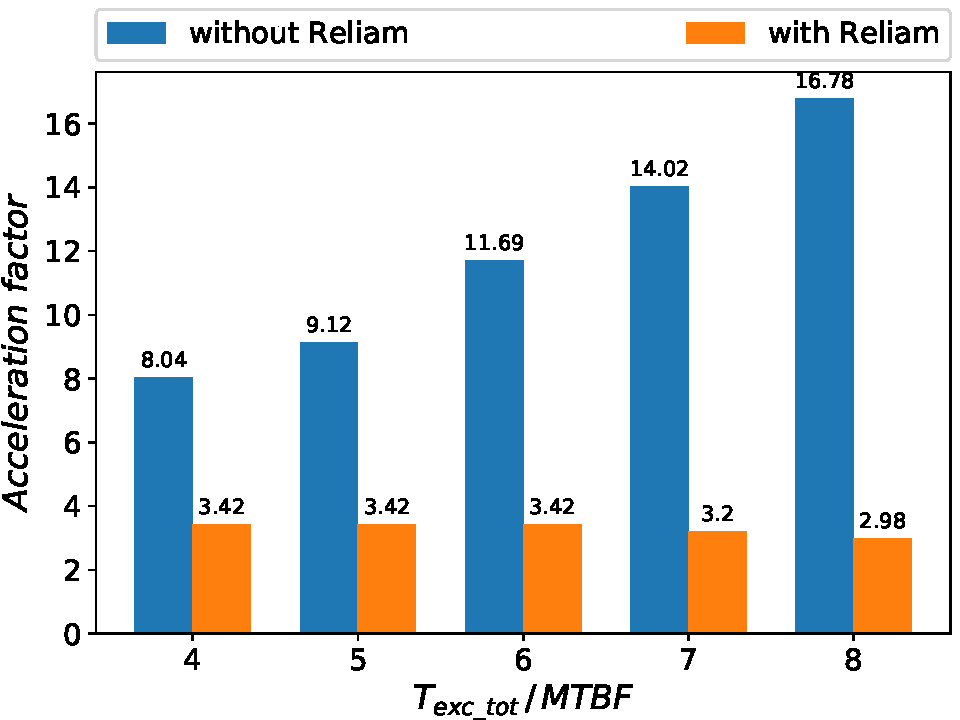
\includegraphics[width=0.55\textwidth]{af_70.pdf} }}
    \vspace{1.1em}
    \subfloat[\centering Criticality threshold equal to 80\%.]{{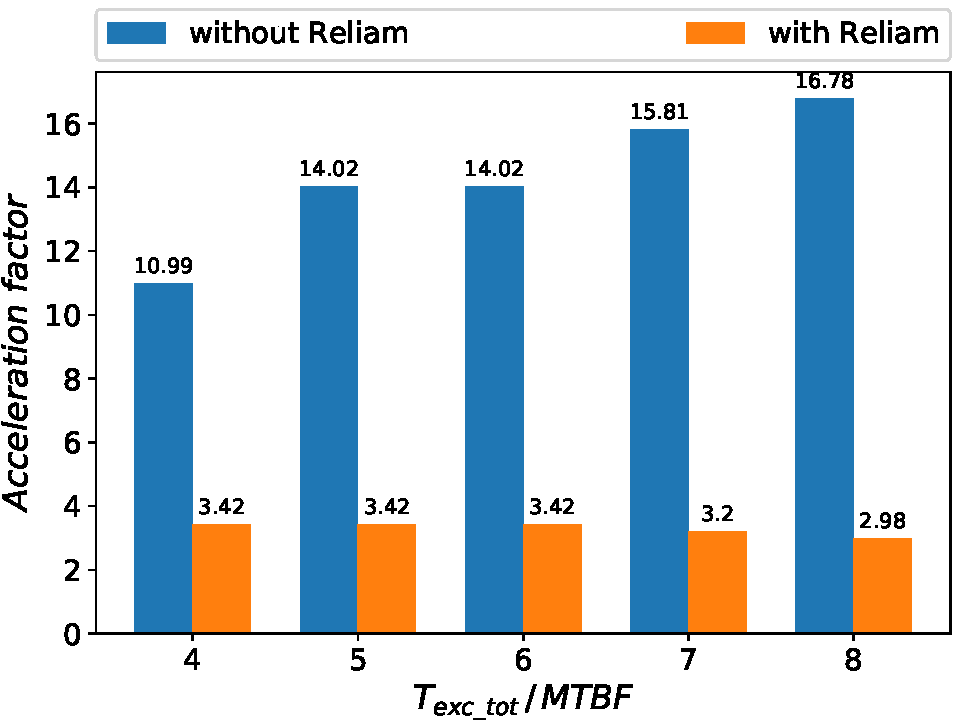
\includegraphics[width=0.55\textwidth]{af_80.pdf} }}
    \caption{Acceleration factor produced by the basic policy (blue bars) and the Reliam Resource Allocation Policy (orange bars).}
    \label{fig:af}%
\end{figure}

 Figure~\ref{fig:af} summarizes the results of such calculation. We can observe the substantial difference between the two curves characterized, respectively, by the absence, in blue, and the presence, in orange, of the reliability control. In the case of criticality threshold equal to 70\%, in the best case, the computed acceleration factor produced without the reliability decisions more than doubles the one observed using it. In the case of criticality threshold equal to 80\%, it more than triples it.  In both plots, in the worst case scenario, represented by $\frac{T_{exc\_tot}}{MTBF}=8$, the acceleration factor produced by the basic policy is higher than the quintuple of the one registered with the Reliam Resource Allocation Policy. 

These results prove the effectiveness of the reliability-aware decisions made by the Reliam Resource Allocation Policy. They not only improve the reliability of the application execution, providing \emph{safer} application-CPU bindings, which lower the probability of using an already worn out processor, but also, slow down the wear out of the hardware components, reducing the acceleration of the reliability degradation in terms of Mean Time To Failure (MTTF) caused by thermal stress.
